\chapter{Feature Implementation and Verification}
\label{chap:implementation}

Chapter~\ref{chap:architecture} introduced the main architectural abstractions of \syssimx{}.
This chapter explains how these abstractions are realized in software and how the implemented features are verified in isolation.
It focuses on implementation decisions that are needed to understand the framework behavior and the case study.
System-level validation is deferred to Chapter~\ref{chap:case_study}.

The chapter is organized along the execution path of a co-simulation scenario.
Section~\ref{sec:impl_port_system} introduces the typed and unit-aware port system.
Section~\ref{sec:impl_component_interface} describes the common component lifecycle and runtime contract.
Section~\ref{sec:impl_wrappers} explains how FMI, OpenSim, and finite-element models are adapted to this contract.
Section~\ref{sec:impl_system} describes system assembly, signal connections, event connections, and lifecycle orchestration.

The following sections cover the execution logic built on top of the registered system.
Section~\ref{sec:impl_structural} derives the structural metadata used for initialization and stepping.
Section~\ref{sec:impl_algebraic_loops} describes the local resolution of algebraic loops.
Section~\ref{sec:impl_algorithms} presents the continuous master algorithms.
Section~\ref{sec:impl_hybrid} extends the stepping logic with event detection, event localization, and dense-time event handling.
Section~\ref{sec:impl_multi_model} describes runtime switching between interchangeable internal models.

\section{Port System}
\label{sec:impl_port_system}

This section describes the typed and unit-aware port system used by all \texttt{CoSimComponent} instances.
It realizes \ref{req:SR-01-01} under \ref{req:UR-01} and \ref{req:SR-02-01}--\ref{req:SR-02-03} under \ref{req:UR-02}.
The implementation provides the port interface introduced in Section~\ref{sec:architecture_cosimcomponent}.
The same machinery supports connection validation, value propagation, history recording, and event-port creation.

%%%%%%%%%%%%%%%%%%%%%%%%%%%%%%%%%%%%%%%%%%%%%%%%%%%%%%
\subsection{Specification and State}

The implementation separates the static port specification from the mutable runtime value, as shown in Figure~\ref{fig:impl_port_system}.
The \texttt{PortSpec} class defines the interface contract of a port.
The \texttt{PortState} class stores the current value and validates every runtime update against this contract.

\begin{figure}[htbp]
  \centering
  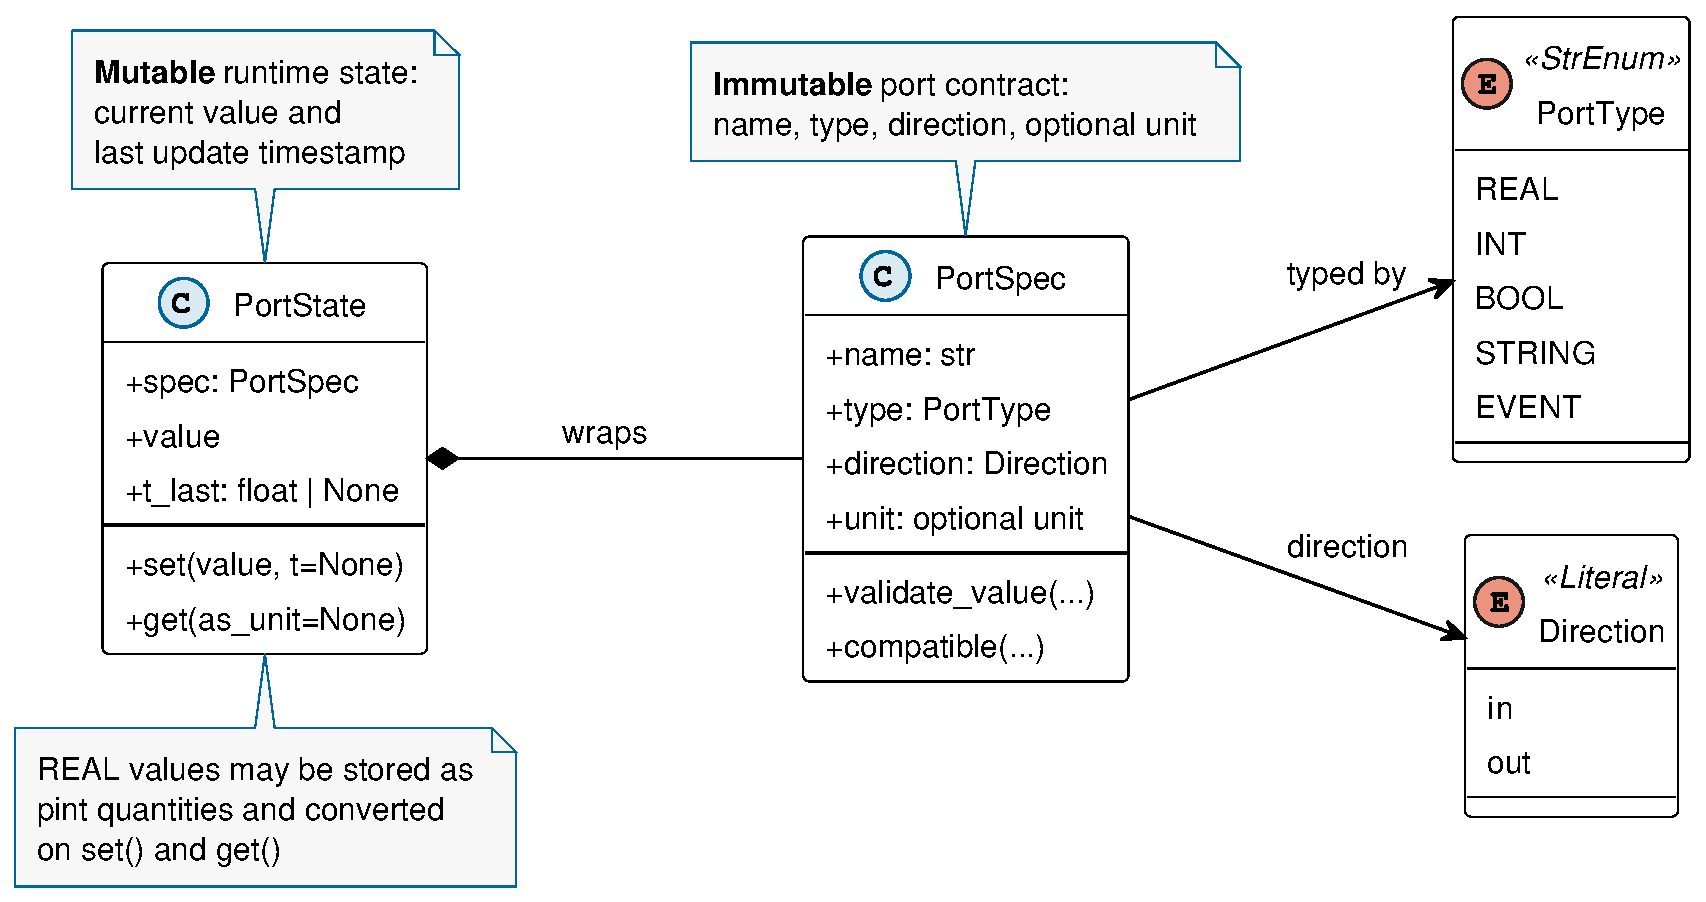
\includegraphics[width=0.75\linewidth]{diagrams/out/pdf/class/core/Port.pdf}
  \caption[Class diagram of the port system]{Class diagram of the port system.
  The \texttt{PortSpec} class defines the immutable port contract.
  The \texttt{PortState} class stores the runtime value and applies type and unit validation.}
  \label{fig:impl_port_system}
\end{figure}

\paragraph{Port Types.}
Table~\ref{tab:impl_port_types} lists the supported data types.
They are implemented by the \texttt{PortType} enumeration.
Physical units are allowed only for \texttt{REAL} ports.
The \texttt{EVENT} type represents boolean trigger ports.
Such ports are created automatically for registered event indicators during component initialization, as described in Section~\ref{sec:impl_component_interface}.

\begin{table}[htbp]
  \centering
  \small
  \caption{Supported port data types in the \texttt{PortType} enumeration.}
  \label{tab:impl_port_types}
  \begin{tabular}{lll}
    \toprule
    \textbf{Type}   & \textbf{Python value}                    & \textbf{Unit allowed} \\
    \midrule
    \texttt{REAL}   & \texttt{float} or \texttt{pint.Quantity} & yes                   \\
    \texttt{INT}    & \texttt{int}                             & no                    \\
    \texttt{BOOL}   & \texttt{bool}                            & no                    \\
    \texttt{STRING} & \texttt{str}                             & no                    \\
    \texttt{EVENT}  & \texttt{bool} (trigger)                  & no                    \\
    \bottomrule
  \end{tabular}
\end{table}

\paragraph{Port Specification.}
A \texttt{PortSpec} is a frozen dataclass that describes one port.
It stores the port name, direction, data type, optional physical unit, and an optional description.
Unit strings are validated against the shared Pint registry during construction.
Malformed specifications are therefore rejected before a component is instantiated.

The static method \pyfn{PortSpec.compatible()} defines the connection rule used by the \texttt{System} class.
Two specifications are compatible when their data types match exactly.
For \texttt{REAL} ports, both ports must either be dimensionless or carry dimensionally compatible units.
This rule is consumed during connection registration in \pyfn{System.\_validate\_connection()} (Section~\ref{sec:impl_system}).

\paragraph{Port State.}
A \texttt{PortState} stores the current value of one port and the time of the last update.
It references the corresponding \texttt{PortSpec}.
On \texttt{set()}, the value is checked against the specification.
For \texttt{REAL} ports, compatible quantities are converted to the declared port unit.
On \texttt{get()}, callers may request a target unit.
This allows downstream code to read values in a convenient unit while preserving dimensional information.
Port states are instantiated from the registered specifications during component initialization.

%%%%%%%%%%%%%%%%%%%%%%%%%%%%%%%%%%%%%%%%%%%%%%%%%%%%%%
\subsection{Physical Unit Handling}
\label{sec:impl_units}

Physical units are handled through Pint~\cite{grecco_pint_nodate}.
The framework uses one shared unit registry for all ports and components.
Unit checks occur at three points.
First, unit strings are validated when a \texttt{PortSpec} is constructed.
Second, \texttt{System.\_validate\_connection()} checks dimensional compatibility between connected ports through \texttt{PortSpec.compatible()}.
Third, \texttt{PortState.set()} converts incoming values to the declared port unit and rejects incompatible dimensions.

FMI~2.0 FMUs exported from OpenModelica may use compact unit strings such as \texttt{"m.s-2"} for $\mathrm{m}\,\mathrm{s}^{-2}$.
These strings are normalized before they are passed to Pint.
This keeps the public port interface consistent even when backend tools use different unit-string conventions.

%%%%%%%%%%%%%%%%%%%%%%%%%%%%%%%%%%%%%%%%%%%%%%%%%%%%%%
\subsection{Verification}

The port-system verification checks the acceptance and rejection behavior of the runtime value layer.
The representative cases in Table~\ref{tab:port_verification} cover type validation, unit compatibility, automatic conversion, and FMI unit-string normalization.
Together, these cases confirm that invalid values and incompatible connections are rejected before they can affect a simulation run.

\begin{table}[htbp]
  \centering
  \small
  \caption{Acceptance and rejection cases for port values and port connections.}
  \label{tab:port_verification}
  \begin{tabular}{lll}
    \toprule
    \textbf{Operation}                       & \textbf{Input}     & \textbf{Result}                     \\
    \midrule
    Set REAL port (\texttt{m/s})             & \texttt{3.6\,km/h} & converted to \texttt{1.0\,m/s}      \\
    Set REAL port (\texttt{rad})             & \texttt{42} (int)  & accepted as \texttt{42.0\,rad}      \\
    Set REAL port (\texttt{m/s})             & \texttt{"hello"}   & rejected (\texttt{TypeError})       \\
    Connect \texttt{m/s} $\to$ \texttt{km/h} & n/a                & compatible (same dimension)         \\
    Connect \texttt{m/s} $\to$ \texttt{N}    & n/a                & incompatible (different dimension)  \\
    Connect \texttt{REAL} $\to$ \texttt{INT} & n/a                & incompatible (type mismatch)        \\
    Normalize FMI unit string                & \texttt{"m.s-2"}   & parsed as $\text{m}\,\text{s}^{-2}$ \\
    \bottomrule
  \end{tabular}
\end{table}
\section{Component Interface}
\label{sec:impl_component_interface}

The \texttt{CoSimComponent} base class implements the common runtime contract for all simulation components in \syssimx{}.
It realizes the component abstraction introduced in Section~\ref{sec:architecture_cosimcomponent} and builds on the port system of Section~\ref{sec:impl_port_system}.
The class centralizes lifecycle control, port-state management, history recording, and common structural and hybrid metadata.
Backend wrappers therefore only implement the model-specific operations.

%%%%%%%%%%%%%%%%%%%%%%%%%%%%%%%%%%%%%%%%%%%%%%%%%%%%%%
\subsection{Design}

\texttt{CoSimComponent} is implemented as an abstract base class that follows the template method pattern~\cite{gamma_design_1995}.
The public lifecycle methods define a fixed execution skeleton.
Primitive operations provide the mandatory subclass-specific behavior.
Hook operations extend the contract for features such as state transfer, rollback, zero-step output evaluation, and event handling.
Table~\ref{tab:component_methods} summarizes this organization.

%
\begin{table}[!htbp]
  \centering
  \small
  \caption{Role-based classification of the main \texttt{CoSimComponent} methods.
  Template methods define the public lifecycle.
  Primitive operations are implemented by each subclass.
  Hook operations provide optional extension points.}
  \label{tab:component_methods}
  \begin{tabular}{llp{5.8cm}}
    \toprule
    \textbf{Method} & \textbf{Contract} & \textbf{Purpose} \\
    \midrule
    \texttt{initialize(t0)}                              & Template  & Component lifecycle startup \\
    \texttt{do\_step(t, dt)}                             & Template  & Macro time step \\
    \texttt{handle\_event(event\_names, t)}              & Template  & Event handling and output refresh \\
    \midrule
    \texttt{\_initialize\_component(t0)}                 & Primitive & Component-specific initialization \\
    \texttt{\_do\_step\_internal(t, dt)}                 & Primitive & Time step computation \\
    \texttt{\_update\_output\_states(t)}                 & Primitive & Write internal state to output ports \\
    \midrule
    \texttt{get\_state() / set\_state()}                 & Hook      & Physical state transfer \\
    \texttt{snapshot\_state() / restore\_state()}        & Hook      & Opaque state rollback \\
    \texttt{evaluate\_outputs(inputs, t)}                & Hook      & Zero-step output evaluation \\
    \texttt{\_handle\_events\_internal(event\_names, t)} & Hook      & Event-driven state update \\
    \texttt{reset()}                                     & Hook      & Clear state \\
    \bottomrule
  \end{tabular}
\end{table}

This organization inverts the control flow.
The master algorithm calls a template method on the base class.
The base class then delegates only the model-specific part to the subclass.
This keeps time bookkeeping, output refresh, history recording, and capability checks consistent across all backend wrappers.

%%%%%%%%%%%%%%%%%%%%%%%%%%%%%%%%%%%%%%%%%%%%%%%%%%%%%%
\subsection{Runtime State}

Each component is identified by a unique \texttt{name}.
The \texttt{System} uses this name for connection definitions, graph construction, error messages, and history labels.
An optional \texttt{group} assigns the component to a display group used by the system graph visualizer.

The port interface is represented at two levels.
The immutable specifications \texttt{input\_specs} and \texttt{output\_specs} are declared by the subclass during construction.
The mutable port states \texttt{inputs} and \texttt{outputs} are created from these specifications during initialization.
They store the runtime values exchanged during simulation.

The current simulation time is stored in \texttt{t}.
The flag \texttt{\_is\_initialized} prevents repeated initialization from modifying an already initialized component.
The \texttt{history} object records time-stamped output values after initialization, after each step, and after event handling.
This supports the result-export requirement discussed in Section~\ref{sec:req_interaction}.

The \texttt{direct\_feedthrough} attribute stores algebraic input-output dependencies.
It is populated during initialization and consumed by the structural analysis of Section~\ref{sec:impl_structural}.
Hybrid components add event indicators and event subscriptions.
The hybrid algorithm consumes this metadata during event detection and event dispatch.

%%%%%%%%%%%%%%%%%%%%%%%%%%%%%%%%%%%%%%%%%%%%%%%%%%%%%%
\subsection{Lifecycle Semantics}

\paragraph{Construction.}
A concrete subclass first calls \texttt{super().\_\_init\_\_()}.
The base constructor allocates the containers for ports, parameters, history, structural metadata, and hybrid metadata.
The subclass then declares its input and output specifications.
It may also declare default parameters and event indicators.

\paragraph{Configuration.}
A component is configured through \texttt{set\_parameters()} before initialization.
The method validates keyword arguments against the parameter dictionary of the component.
Subclasses define the available parameters and their default values.
The actual backend-specific application of these parameters happens during \texttt{\_initialize\_component()}.

\paragraph{Initialization.}
The initialization sequence is shown in Figure~\ref{fig:impl_comp_initialization}.
The template method \texttt{initialize(t0)} is idempotent.
If the component is already initialized, it returns without changing the runtime state.
Otherwise, the base class stores the initial time and creates the regular port states from the declared specifications.
It also creates event output ports for indicators that were registered before initialization.

The method then delegates model-specific setup to \texttt{\_initialize\_component(t0)}.
After this step, the base class detects direct feedthrough dependencies, publishes the initial outputs through \texttt{\_update\_output\_states(t0)}, records them in the component history, and marks the component as initialized.

\begin{figure}[btbp]
  \centering
  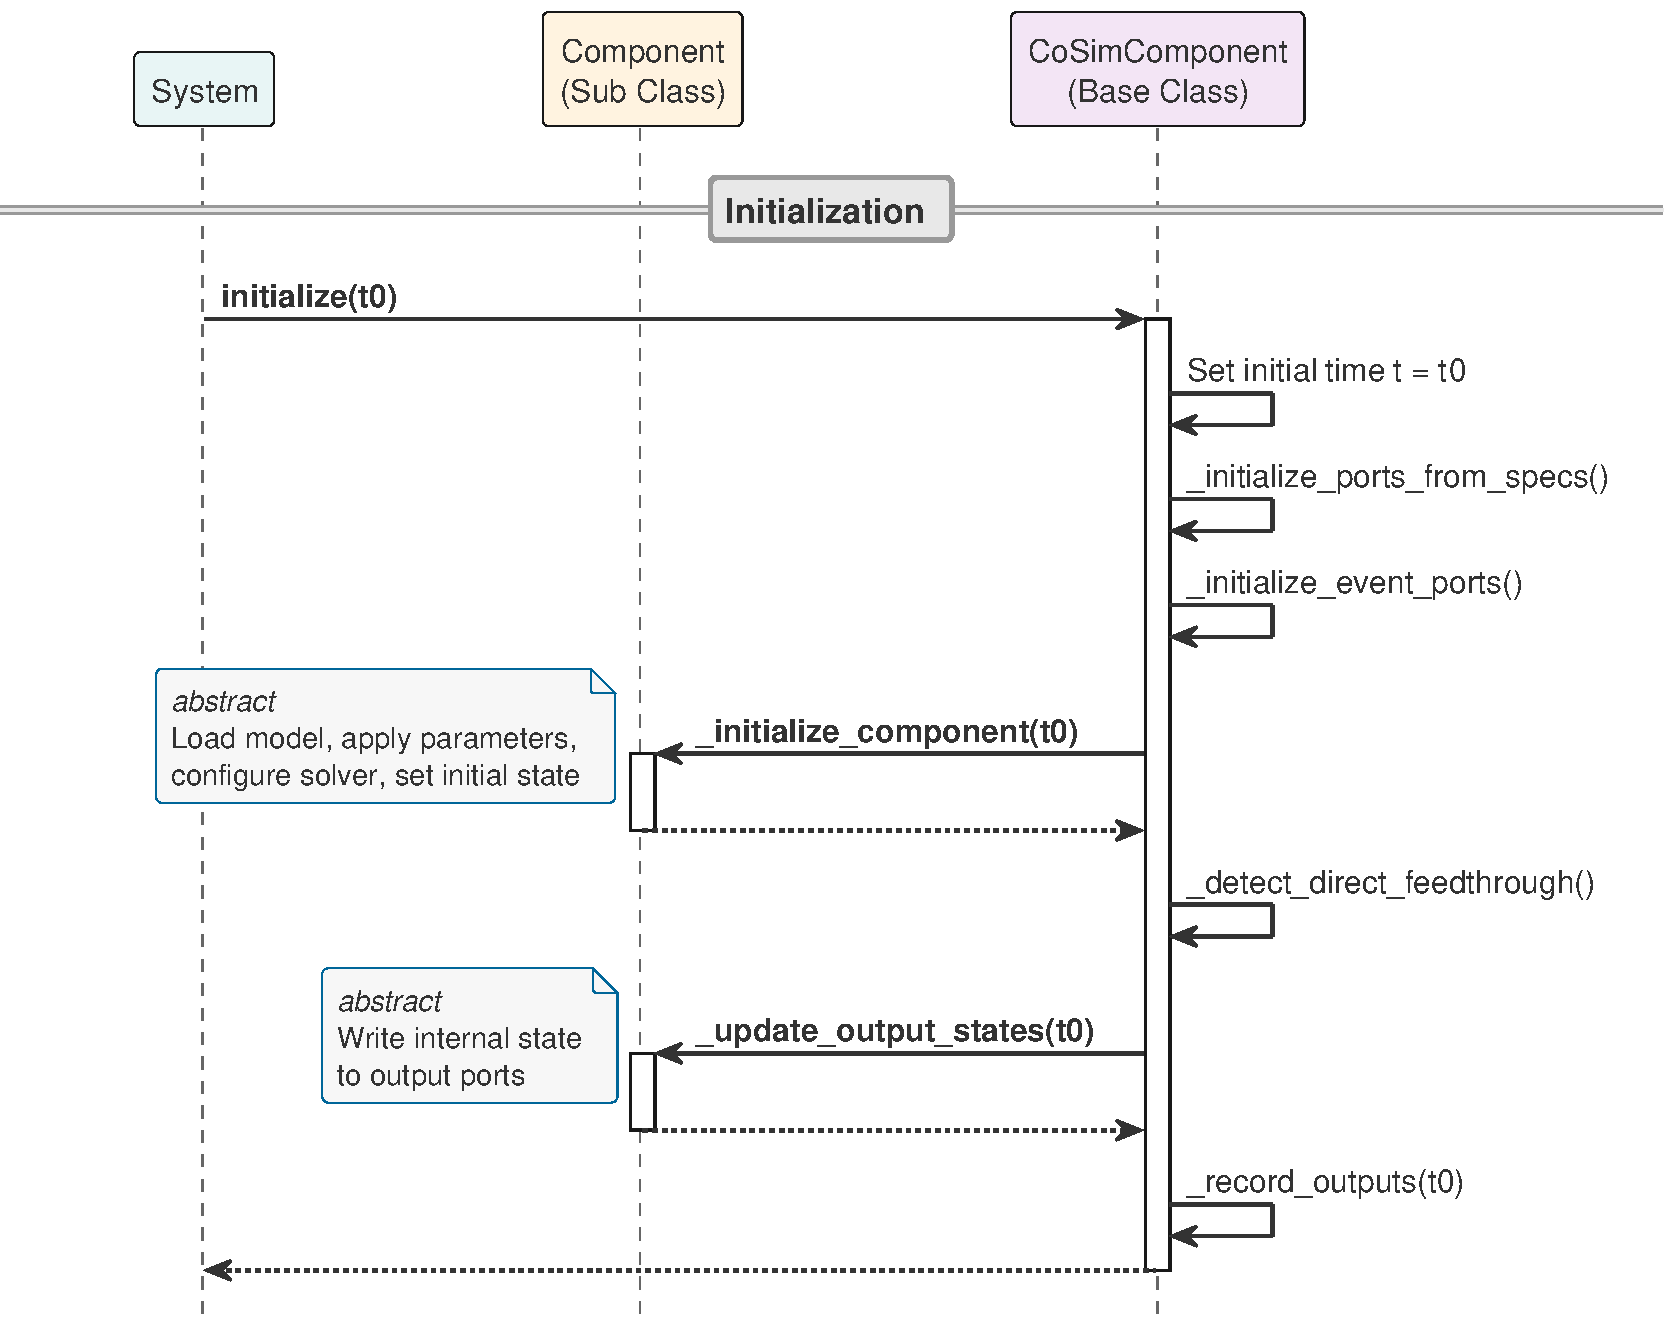
\includegraphics[width=0.8\linewidth]{diagrams/out/pdf/execution/CoSimComponent_Initialization.pdf}
  \caption{Delegation during component initialization. The template method
    \texttt{initialize()} performs the idempotency check, creates regular
    and event ports, delegates model-specific setup to
    \texttt{\_initialize\_component()}, detects direct feedthrough, publishes
    initial outputs through \texttt{\_update\_output\_states()}, and records
    the initial output values.}
  \label{fig:impl_comp_initialization}
\end{figure}

\paragraph{Simulation Step.}
Figure~\ref{fig:impl_comp_stepping} shows one macro step.
The master algorithm calls \texttt{do\_step(t,dt)}.
The template method delegates the numerical advancement to \texttt{\_do\_step\_internal()}.
After the subclass returns, the base class updates \texttt{t}, refreshes the output ports, and records the new output values.

\begin{figure}[btbp]
  \centering
  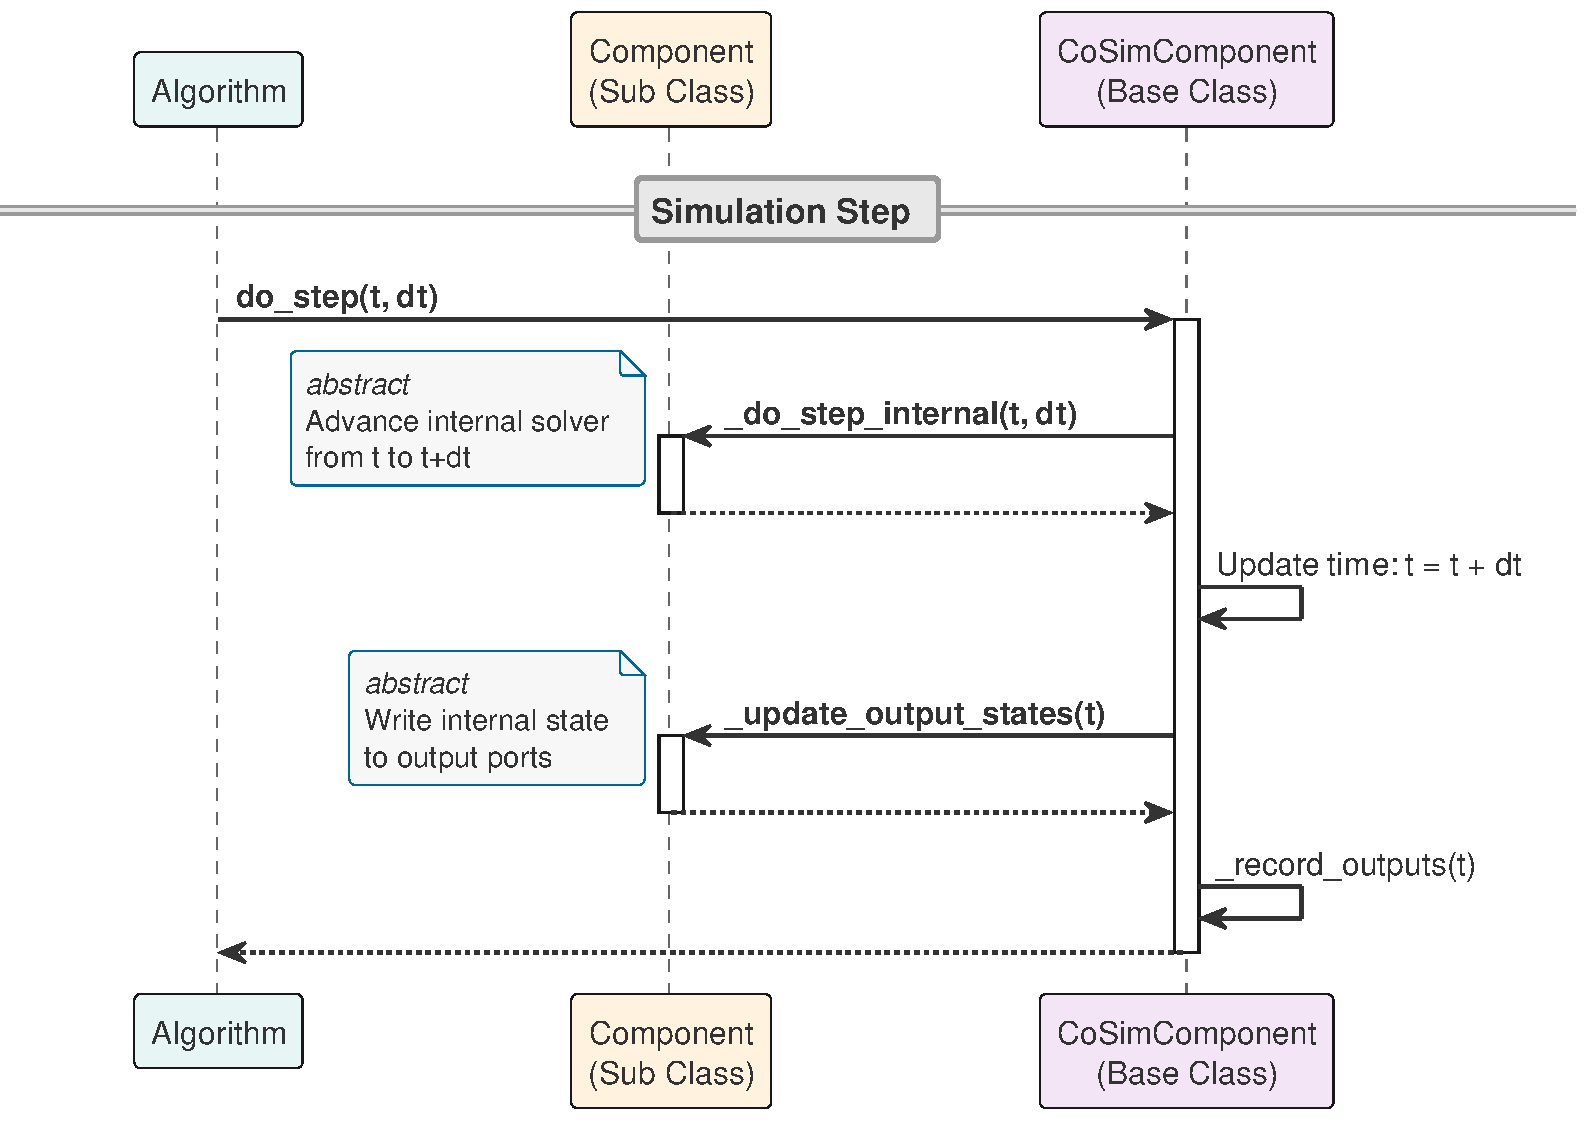
\includegraphics[width=0.8\linewidth]{diagrams/out/pdf/execution/CoSimComponent_Stepping.pdf}
  \caption{Delegation during a simulation step. The template method
    \texttt{do\_step()} delegates the computation to the primitive operation
    \texttt{\_do\_step\_internal()} and the output update to
    \texttt{\_update\_output\_states()}.}
  \label{fig:impl_comp_stepping}
\end{figure}

\paragraph{Event Handling.}
The template method \pyfn{handle\_event(event\_names,\,t)} is called by the hybrid algorithm at event times (Section~\ref{sec:impl_hybrid}).
It delegates the state update to the hook operation \pyfn{\_handle\_events\_internal()}, then calls \pyfn{\_update\_output\_states()} to refresh the output ports, and records the updated values in the component history.
Components that do not participate in hybrid simulation inherit an empty default for \pyfn{\_handle\_events\_internal()}, so the call is a no-op.

\paragraph{Reset and Cleanup.}
After the simulation loop, the hook operation \pyfn{reset()} supports component reuse.
It clears the simulation time, history buffer, and initialization flag, allowing the component to be re-initialized with \pyfn{initialize()} for a new run.
Subclasses extend the default implementation via \pyfn{super().reset()} to
additionally clear internal state.

%%%%%%%%%%%%%%%%%%%%%%%%%%%%%%%%%%%%%%%%%%%%%%%%%%%%%%
\subsection{Verification}

The verification of \texttt{CoSimComponent} targets framework-level invariants that are independent of any backend.
Lightweight mock subclasses, such as a pure-gain feedthrough component, a simple integrator, and minimal hybrid components, implement only the three primitive operations, keeping the tests focused on base-class behavior.

Table~\ref{tab:cosimcomp_verification} summarizes the verified base-class invariants.

\begin{table}[htbp]
  \centering
  \small
  \caption{Verification of the main \texttt{CoSimComponent} base-class invariants.}
  \label{tab:cosimcomp_verification}
  \begin{tabular}{p{5.8cm} p{8.2cm}}
    \toprule
    \textbf{Verified invariant} & \textbf{Expected outcome} \\
    \midrule
    Initialization lifecycle
      & \texttt{initialize()} creates port states, delegates model setup once, publishes initial outputs, records history, and remains idempotent \\
    \addlinespace
    Step lifecycle
      & \texttt{do\_step()} delegates numerical advancement, updates time, refreshes outputs, and records the stepped values \\
    \addlinespace
    Direct-feedthrough detection
      & Feedthrough components report algebraic input-output dependencies, while pure integrators report none \\
    \addlinespace
    Reset lifecycle
      & \texttt{reset()} clears time, history, and initialization state so that the component can be initialized again \\
    \addlinespace
    Event-port handling
      & Event output ports are created for registered event indicators before or after initialization \\
    \bottomrule
  \end{tabular}
\end{table}

The tests confirm that the base class enforces the component contract independently of any backend.
The template methods create port states, preserve lifecycle order, update output values, and record history consistently.
The feedthrough detector identifies algebraic dependencies for feedthrough components and leaves pure integrators without feedthrough.
Backend-specific hook behavior is verified in the corresponding wrapper sections because its correctness depends on the concrete model semantics.
%%%%%%%%%%%%%%%%%%%%%%%%%%%%%%%%%%%%%%%%%%%%%%%%%%%%%%%%%%%%%%%%
\section{Component Wrappers}
\label{sec:impl_wrappers}

\subsection{FMI 2.0 Co-Simulation Wrapper}
\label{sec:impl_fmu}

The \texttt{FMUComponent} wrapper maps \ac{FMI}~2.0 Co-Simulation \acp{FMU} to the \texttt{CoSimComponent} interface of Section~\ref{sec:impl_component_interface}.
It realizes \ref{req:SR-05-01} under \ref{req:UR-05}.
The wrapper delegates \ac{FMI} calls to \texttt{fmpy}~\cite{dassault_systemes__catia-systems_fmpy_2026}.
It derives ports, parameters, value references, and direct-feedthrough metadata from the model description of the \ac{FMU}.

As described in Section~\ref{sec:237_cosim_fmi}, a Co-Simulation \ac{FMU} advances its model with an internal solver.
The \texttt{FMUComponent} class exposes this solver-owned simulation unit through the \syssimx{} component contract.
The resulting component can be connected, initialized, stepped, and inspected like any other \texttt{CoSimComponent}.

%%%%%%%%%%%%%%%%%%%%%%%%%%%%%%%%%%%%%%%%%%%%%%%%%%%%%%
\subsubsection{Architecture and Interface Mapping}

Figure~\ref{fig:impl_fmu_class} shows how the \ac{FMU} wrapper connects the framework contract to the \ac{FMI} runtime object.
The \texttt{FMUComponent} class inherits the template methods and port machinery from \texttt{CoSimComponent}.
It stores the \texttt{FMU2Slave} instance provided by \texttt{fmpy} as the backend object that executes \ac{FMI} calls.

\begin{figure}[t]
  \centering
  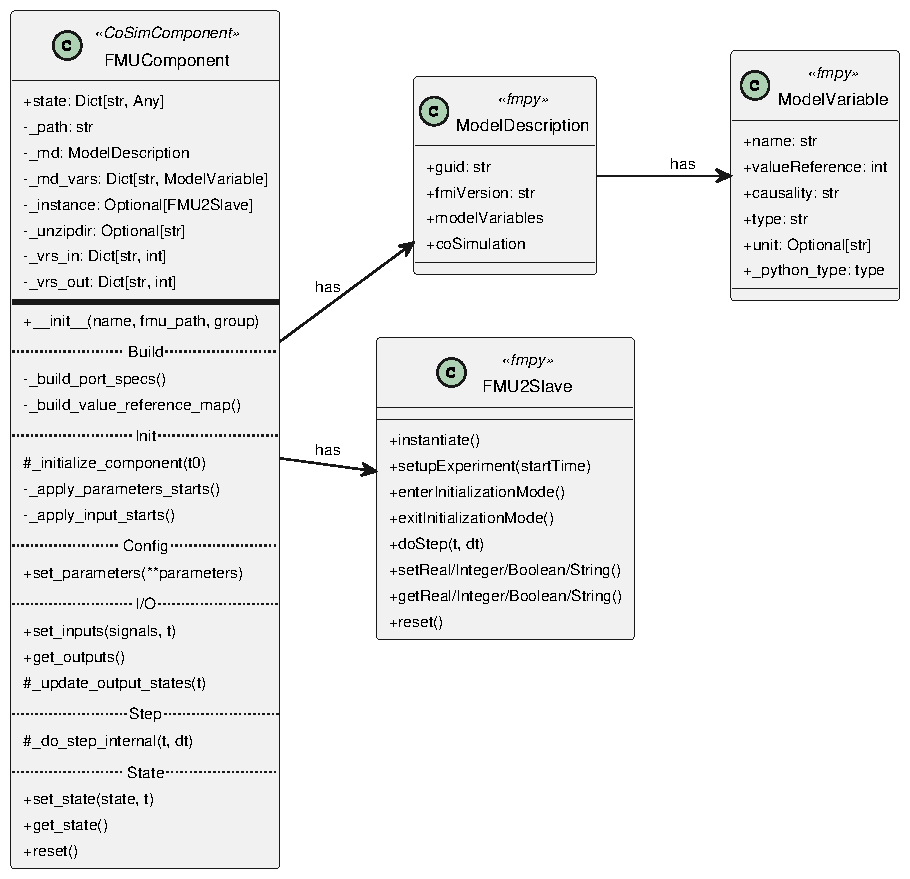
\includegraphics[width=\linewidth]{diagrams/out/pdf/class/components/FMUComponent.pdf}
  \caption[Class diagram of the \ac{FMU} wrapper]{Class diagram of the \ac{FMU} wrapper.
  The \texttt{FMUComponent} class adapts an \ac{FMI}~2.0 Co-Simulation \ac{FMU} to the \texttt{CoSimComponent} contract.
  The parsed model description supplies ports, parameters, value references, and direct-feedthrough metadata.
  The \texttt{FMU2Slave} instance executes the \ac{FMI} runtime operations.}
  \label{fig:impl_fmu_class}
\end{figure}

During construction, the wrapper parses the \ac{FMU} model description once.
It uses this metadata to create the \syssimx{}-level component interface.
Table~\ref{tab:fmu_mapping} lists the correspondence between \ac{FMI} artefacts and the component abstractions of Sections~\ref{sec:impl_port_system} and~\ref{sec:impl_component_interface}.

\begin{table}[t]
  \centering
  \small
  \caption[Mapping from \ac{FMI} model-description artefacts to \syssimx{} abstractions]{Mapping from \ac{FMI}~2.0 model-description artefacts to \syssimx{} component abstractions.
  The \texttt{FMUComponent} class computes this mapping once during construction.}
  \label{tab:fmu_mapping}
  \begin{tabular}{@{}p{0.42\linewidth}p{0.54\linewidth}@{}}
    \toprule
    \textbf{\ac{FMI} artefact} & \textbf{\syssimx{} abstraction} \\
    \midrule
    \texttt{ScalarVariable} with causality \texttt{input} or \texttt{output}
      & \texttt{PortSpec} with matching direction, data type, unit, and description \\
    \addlinespace
    \texttt{ScalarVariable} with causality \texttt{parameter}, \texttt{calculatedParameter}, or \texttt{structuralParameter}
      & Entry in the component's \texttt{parameters} dictionary with converted start value \\
    \addlinespace
    \texttt{ModelStructure/Outputs} dependencies
      & Entries in the \texttt{direct\_feedthrough} dictionary \\
    \addlinespace
    \texttt{valueReference}
      & Cached input and output reference maps grouped by \ac{FMI} base type \\
    \addlinespace
    \ac{FMI} unit strings such as \texttt{"m.s-2"}
      & Pint-compatible units on \texttt{REAL} ports after unit-string normalization \\
    \bottomrule
  \end{tabular}
\end{table}

The value-reference maps are cached once during construction.
\ac{FMI} variables are accessed by integer value references rather than by name.
The cached references are used for batched input writes and output reads grouped by \ac{FMI} base type.
This keeps runtime access independent of repeated name lookups.

Generic components use perturbation-based feedthrough detection, as described in Section~\ref{sec:impl_component_interface}.
\acp{FMU} can declare output dependencies in the \texttt{ModelStructure} element of the model description.
The \texttt{FMUComponent} class reads these dependencies directly and stores them in the feedthrough metadata.
This avoids additional \ac{FMI} calls and uses the dependencies declared by the \ac{FMU} exporter.

%%%%%%%%%%%%%%%%%%%%%%%%%%%%%%%%%%%%%%%%%%%%%%%%%%%%%%
\subsubsection{Lifecycle Realization}

The \texttt{FMUComponent} class realizes the primitive operations of the \texttt{CoSimComponent} base class through \ac{FMI}~2.0 calls.
During initialization, the wrapper extracts the \ac{FMU} archive and instantiates the \texttt{FMU2Slave}.
It calls \texttt{setupExperiment()}, enters initialization mode, applies parameters and input start values, and exits initialization mode.
The base-class template then publishes the initial outputs and records them in the component history.

A macro step is delegated to the \ac{FMI} \texttt{doStep()} call.
The call receives the current communication point $t$ and the communication step size $\Delta t$.
The base class handles time bookkeeping, output refresh, and history recording around this backend call.
Output refresh uses the cached value references.
The wrapper reads \ac{FMU} outputs through one getter call per active \ac{FMI} base type.
For \texttt{REAL} outputs, the declared unit is attached before the value is written to the corresponding \texttt{PortState}.

The hook \texttt{evaluate\_outputs(inputs, t)} supports algebraic-loop resolution.
It applies trial inputs and evaluates the \ac{FMU} outputs without committing a macro step.
The hook is used only for \acp{FMU} that support such zero-step evaluation.
It provides the instantaneous output values required by Section~\ref{sec:impl_algebraic_loops}.


%%%%%%%%%%%%%%%%%%%%%%%%%%%%%%%%%%%%%%%%%%%%%%%%%%%%%%
\subsubsection{State Access and Rollback Boundary}

The \texttt{FMUComponent} class implements the \texttt{get\_state()} and \texttt{set\_state()} methods as part of the framework state-transfer interface.
These methods are distinct from native \ac{FMI} state operations such as \texttt{getFMUState()} and \texttt{setFMUState()}.
The \texttt{get\_state()} method returns non-\texttt{fixed} and non-\texttt{local} \ac{FMU} variables with their current values and declared units.
The \texttt{set\_state()} method uses this dictionary to re-enter initialization, restore serialized values, and refresh the exposed output ports.

This dictionary state is intended for inspection, state transfer, and re-initialization.
Rollback for hybrid event localization requires an opaque snapshot of the internal \ac{FMU} solver state.
The generic \texttt{FMUComponent} only exposes the dictionary state and therefore leaves rollback to specialized subclasses.
Such subclasses can implement rollback when the concrete \ac{FMU} and solver provide a consistent restore mechanism.

%%%%%%%%%%%%%%%%%%%%%%%%%%%%%%%%%%%%%%%%%%%%%%%%%%%%%%
\subsubsection{Verification}

The verification targets the mapping from \ac{FMI} artefacts to the \texttt{CoSimComponent} contract.
The test subject is a purpose-built \ac{FMU} with two real inputs, two real outputs, one boolean parameter, and a declared feedthrough dependency.
Table~\ref{tab:fmu_verification} summarizes the checked properties.

\begin{table}[t]
  \centering
  \small
  \caption[\ac{FMI}-to-component mapping checks]{\ac{FMI}-to-component mapping checks for the purpose-built test \ac{FMU}.}
  \label{tab:fmu_verification}
  \begin{tabular}{p{5.8cm} p{8.8cm}}
    \toprule
    \textbf{Verified property} & \textbf{Expected outcome} \\
    \midrule
    Supported \ac{FMU} type
      & \ac{FMI}~2.0 Co-Simulation \acp{FMU} are accepted, while unsupported \ac{FMI} versions and Model Exchange \acp{FMU} are rejected \\
    \addlinespace
    Interface derivation
      & Ports, parameters, normalized units, and value-reference maps match \texttt{modelDescription.xml} \\
    \addlinespace
    Direct-feedthrough metadata
      & Dependencies declared in \texttt{ModelStructure} are reproduced in \texttt{direct\_feedthrough} \\
    \addlinespace
    Initialization and stepping
      & Parameters and input start values are applied during initialization, and \texttt{do\_step()} advances the \ac{FMU} by one communication step \\
    \addlinespace
    Zero-step output evaluation
      & \texttt{evaluate\_outputs()} returns outputs for supplied interface inputs without committing a macro step \\
    \addlinespace
    Reset and reuse
      & The wrapper can be reset and initialized again for another run \\
    \bottomrule
  \end{tabular}
\end{table}

These properties confirm that the \texttt{FMUComponent} class maps \ac{FMI}~2.0 Co-Simulation \acp{FMU} to the common component contract.
End-to-end integration with control, musculoskeletal, and \ac{FEM} components is evaluated in the controlled-pendulum case study in Chapter~\ref{chap:case_study}.

\subsection{Musculoskeletal Model Wrapper}
\label{sec:impl_opensim}

This subsection describes the implementation of the \texttt{OpenSimComponent} backend wrapper class. It addresses requirement SR-03-02 (integration of musculoskeletal simulation tools) by mapping OpenSim models onto the \texttt{CoSimComponent} interface defined in Section~\ref{sec:impl_component_interface}.
The wrapper delegates all multibody and muscle dynamics to the OpenSim library, which itself builds on the Simbody multibody engine, and encapsulates the realize-integrate cycle behind the primitive and hook operations of the component contract.

% --- BACKGROUND BRIDGE ---
As introduced in Section~\ref{sec:theory_opensim}, an OpenSim model is a Simbody multibody system whose state is advanced by an integrator driven through an \texttt{osim.Manager}.
All derived quantities, such as body positions, forces, muscle activations, generalized accelerations, are obtained from the state through staged realization (\textit{Position},
\textit{Velocity}, \textit{Dynamics}, \textit{Acceleration}).
The wrapper does not re-implement any of this machinery.
Its role is to present an OpenSim model as a \syssimx{} component whose ports, parameters, and lifecycle are aligned with the rest of the framework.

%%%%%%%%%%%%%%%%%%%%%%%%%%%%%%%%%%%%%%%%%%%%%%%%%%%%%%
\subsubsection{Architecture and Interface Mapping}

Figure~\ref{fig:impl_opensim_class} shows the class-level relationship between \texttt{OpenSimComponent}, its abstract base \texttt{CoSimComponent}, and the external OpenSim objects \texttt{Model}, \texttt{Manager}, and \texttt{State}.
Unlike \texttt{FMUComponent} (Section~\ref{sec:impl_fmu}), \texttt{OpenSimComponent} is itself an \emph{abstract base} since OpenSim models do not expose a standardized interface descriptor analogous to \texttt{modelDescription.xml}, so ports, parameters, and the model-assembly steps must be declared by a concrete subclass that targets a specific musculoskeletal model.
The base class provides the infrastructure that is common to every OpenSim component.

\begin{figure}[htbp]
  \centering
  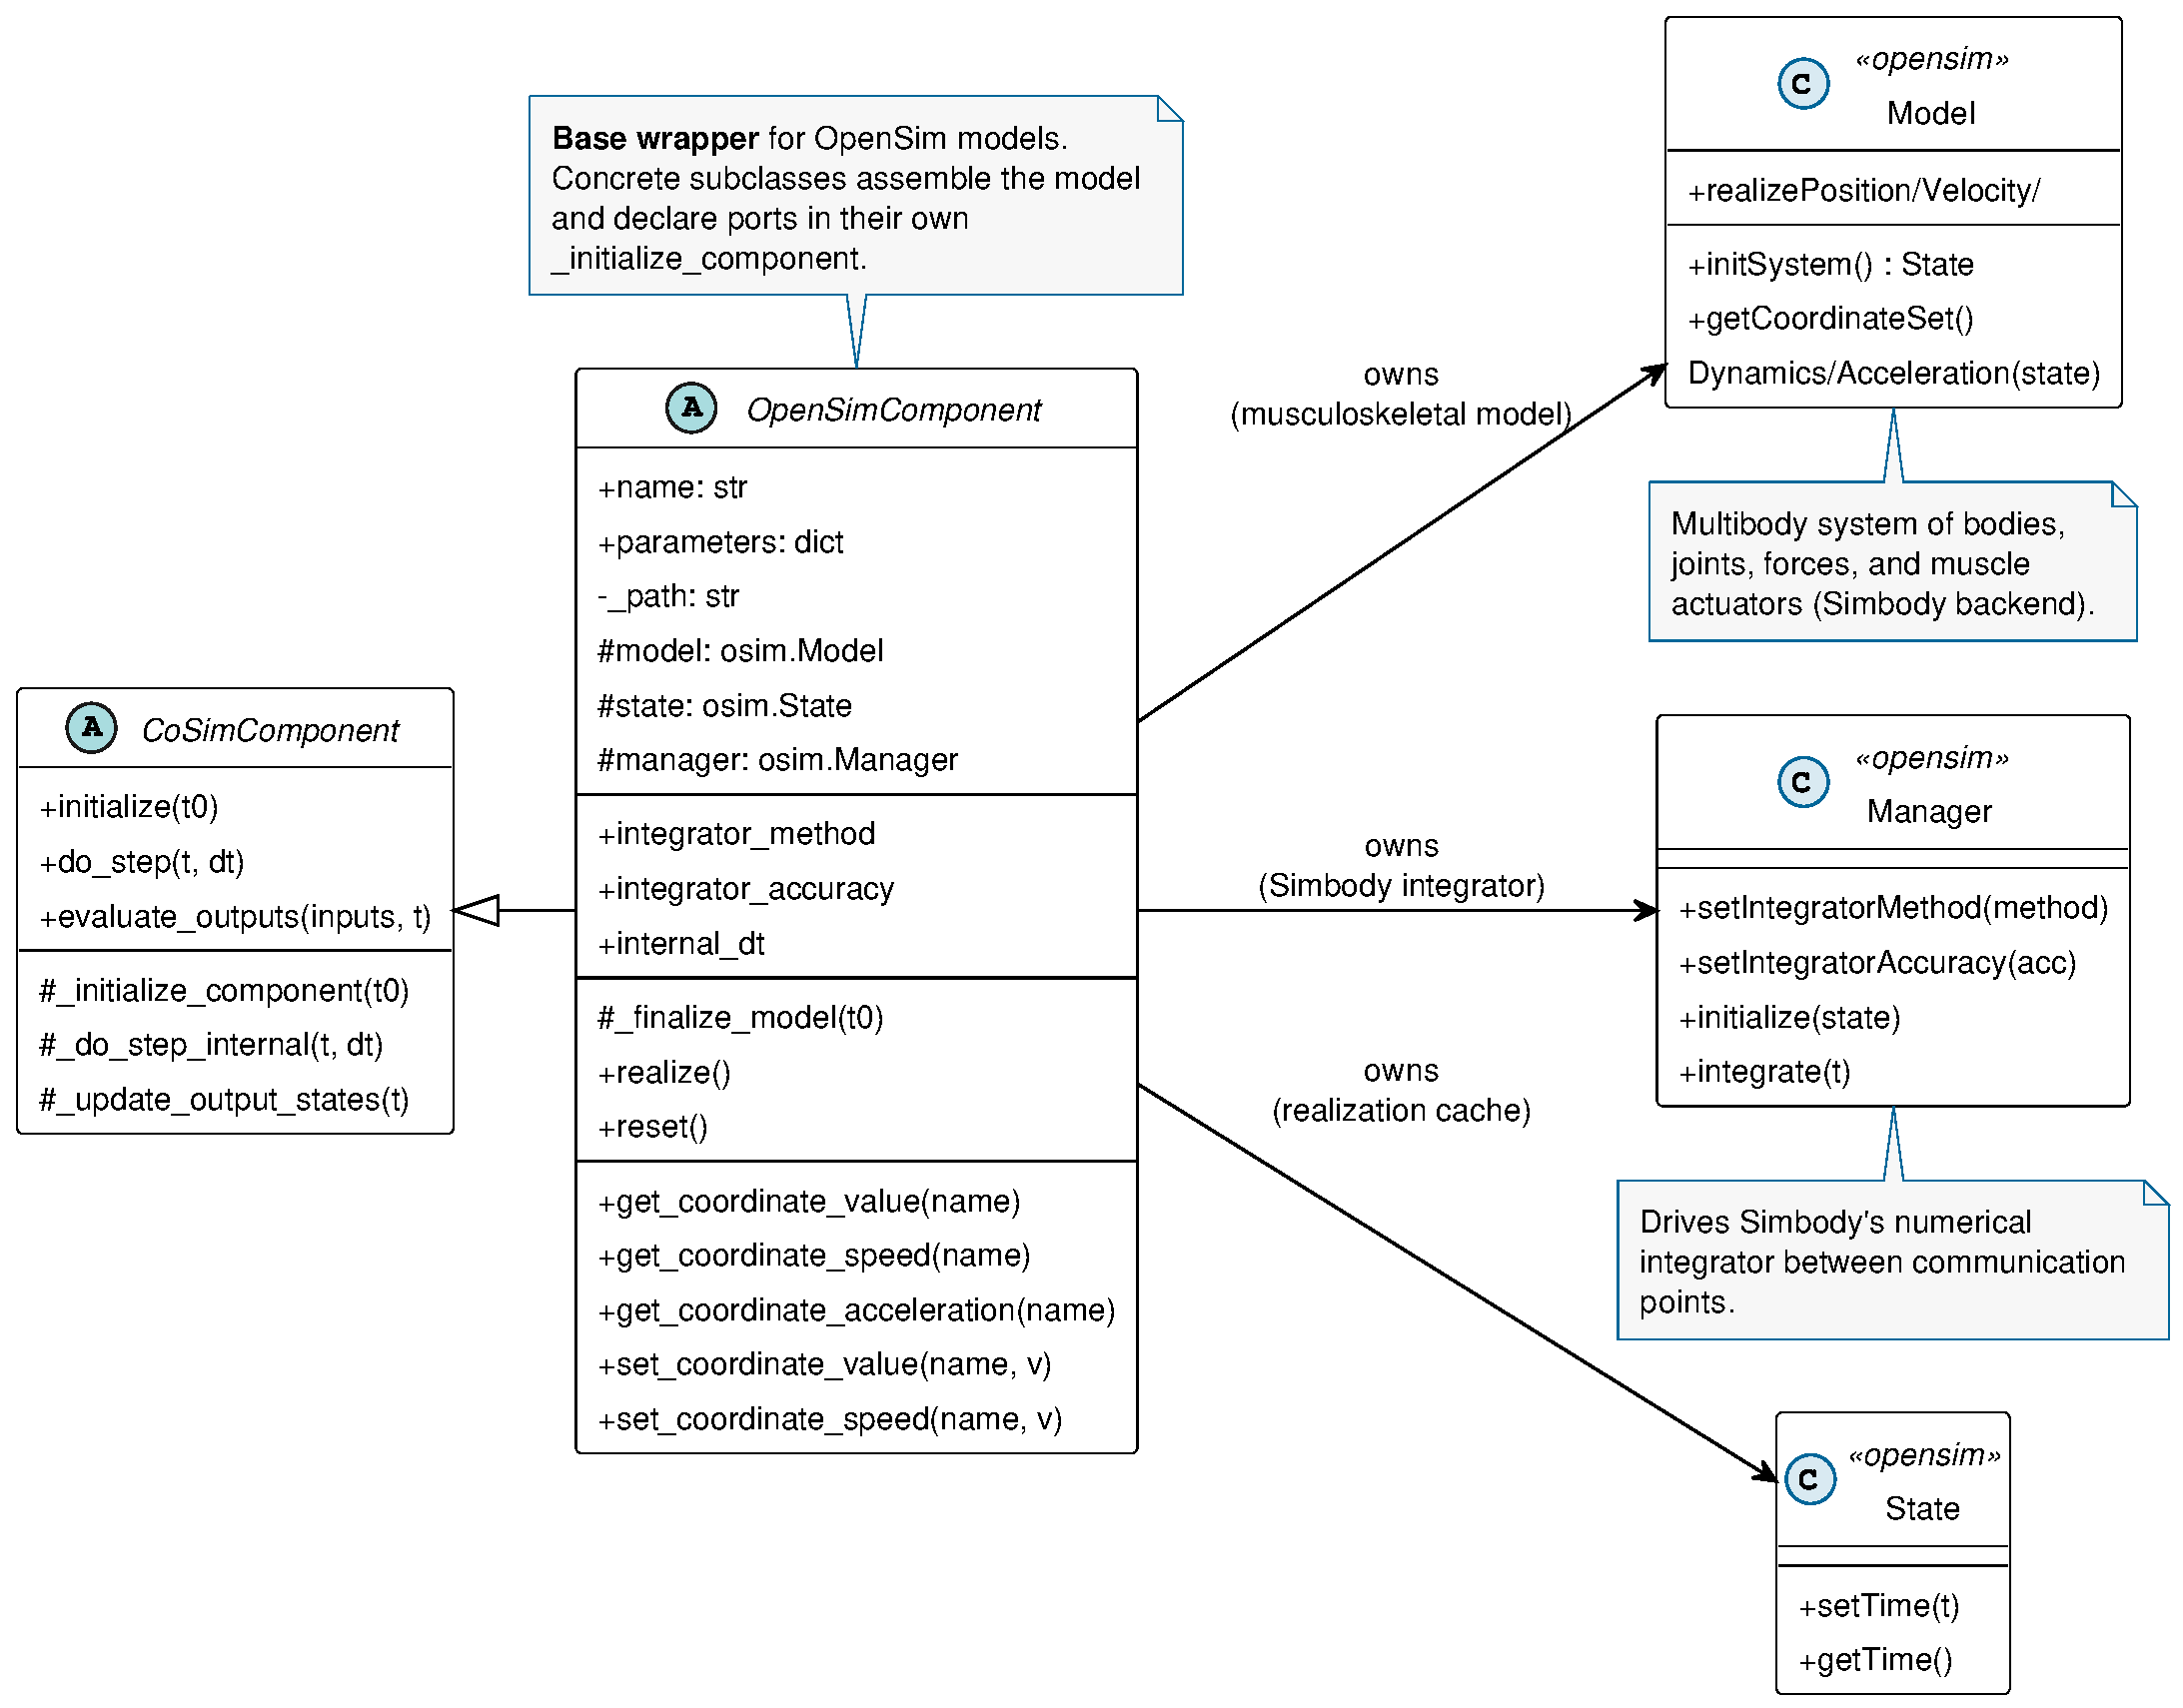
\includegraphics[width=\linewidth]{diagrams/out/pdf/class/components/OpenSimComponent.pdf}
  \caption{Class diagram of the OpenSim wrapper.
           \texttt{OpenSimComponent} specializes
           \texttt{CoSimComponent} and serves as an abstract base for
           concrete musculoskeletal components. It owns an
           \texttt{osim.Model} (multibody system of bodies, joints, forces,
           and muscles), an \texttt{osim.Manager} that drives Simbody's
           integrator, and the associated \texttt{osim.State} that holds
           time, generalized coordinates and velocities, and muscle
           states.}
  \label{fig:impl_opensim_class}
\end{figure}

\paragraph{OpenSim-to-Component Mapping.}
Table~\ref{tab:opensim_mapping} lists the correspondence between OpenSim artefacts and the component abstractions introduced in Sections~\ref{sec:impl_port_system} and \ref{sec:impl_component_interface}.
Unlike the FMU case, the mapping is authored once per concrete subclass rather than derived from a descriptor file.

\begin{table}[htbp]
  \centering
  \small
  \caption{Mapping between OpenSim artefacts and \syssimx{} component
           abstractions. The mapping is established by the concrete
           subclass during construction and initialization.}
  \label{tab:opensim_mapping}
  \begin{tabular}{p{6.3cm} p{7.5cm}}
    \toprule
    \textbf{OpenSim artefact} & \textbf{\syssimx{} abstraction} \\
    \midrule
    \texttt{osim.Model} loaded from a \texttt{.osim} file
      & Backend object owned by the concrete component \\
    \addlinespace
    Selected \texttt{Coordinate} values / speeds
      & \texttt{PortSpec} entries (direction \texttt{in}/\texttt{out}) \\
    \addlinespace
    Muscle activations, control signals, actuator excitations
      & Input \texttt{PortSpec} entries with dimensionless units \\
    \addlinespace
    Body kinematics, muscle forces, generalized accelerations
      & Output \texttt{PortSpec} entries with SI units \\
    \addlinespace
    Model properties set before \texttt{initSystem()}
      & Entries in the component's \texttt{parameters} dictionary \\
    \addlinespace
    Integrator method, accuracy, internal step size
      & Attributes \texttt{integrator\_method},
        \texttt{integrator\_accuracy}, \texttt{internal\_dt} \\
    \bottomrule
  \end{tabular}
\end{table}

\paragraph{Direct-Feedthrough Detection.}
OpenSim does not declare input--output dependencies in a machine-readable form.
\texttt{OpenSimComponent} therefore inherits the default perturbation-based detector from \texttt{CoSimComponent} (Section~\ref{sec:impl_component_interface}). In practice, musculoskeletal
components are almost never feedthrough at the port level as muscle excitations affect activations and forces through differential dynamics, so the corresponding outputs lag the inputs by at least one step.

%%%%%%%%%%%%%%%%%%%%%%%%%%%%%%%%%%%%%%%%%%%%%%%%%%%%%%
\subsubsection*{Lifecycle Realization}

The base class provides the skeleton of the lifecycle and delegates model-specific assembly to the subclass.

\paragraph{Initialization.}
A concrete \texttt{\_initialize\_component(t0)} typically performs the
following steps:
\begin{enumerate}[nosep]
  \item Load the \texttt{.osim} model from the stored path into
        \texttt{self.model}.
  \item Attach any actuators, controllers, or analyses required by the
        port specification.
  \item Apply parameter start values declared on the component.
  \item Call \texttt{self.model.initSystem()} to obtain the initial
        \texttt{osim.State}.
  \item Invoke the inherited helper \texttt{\_finalize\_model(t0)}.
\end{enumerate}
\texttt{\_finalize\_model(t0)} realizes the state through the \textit{Acceleration} stage, instantiates an \texttt{osim.Manager}, configures its integrator method and accuracy, calls \texttt{manager.initialize(state)}, and sets the simulation time to $t_0$.
After the template method \texttt{initialize()} returns, the initial outputs are available in the \texttt{PortState} objects and recorded in the component history.

\paragraph{Stepping.}
\texttt{\_do\_step\_internal(t, dt)} writes the current input ports into the OpenSim state (for example through \texttt{set\_coordinate\_value}/\texttt{set\_coordinate\_speed} or by assigning excitations to controllers) and then issues a single call to \texttt{self.manager.integrate($t+dt$)}. The Simbody integrator advances the state internally with its own adaptive step size, bounded by
\texttt{integrator\_accuracy}.
The communication step $dt$ only defines the boundary at which the coupled simulation synchronizes.

\paragraph{Output Refresh.}
\texttt{\_update\_output\_states()} first calls \texttt{realize()} to
bring the state to the \textit{Acceleration} stage and then reads the port-relevant quantities. Coordinate values, speeds, and accelerations are obtained through the name-based helpers \texttt{get\_coordinate\_value}, \texttt{get\_coordinate\_speed}, and \texttt{get\_coordinate\_acceleration}; muscle and actuator quantities are obtained through the corresponding OpenSim accessor calls.
The results are written back into the \texttt{PortState} objects with their declared units.

\paragraph{Coordinate Helpers.}
The helpers \texttt{get\_coordinate\_*} and \texttt{set\_coordinate\_*} abstract over the \texttt{CoordinateSet} lookup that OpenSim requires for every access and are used by every concrete subclass.
They also serve as the state-transfer primitives used in the multi-model switching
mechanism (Section~\ref{sec:impl_multi_model}), where generalized positions and velocities must be copied between backends whose state representations otherwise differ.

%%%%%%%%%%%%%%%%%%%%%%%%%%%%%%%%%%%%%%%%%%%%%%%%%%%%%%
\subsubsection*{State Access and Rollback Boundary}

The generic \texttt{OpenSimComponent} exposes \texttt{get\_state()} and \texttt{set\_state()} in the same sense as \texttt{FMUComponent}: as a readable dictionary of generalized coordinates, speeds, and activations together with their declared units.
This dictionary is intended for inspection, state transfer across components, and re-initialization.It is not an opaque snapshot of the Simbody integrator.

The method \texttt{reset()} releases the existing \texttt{osim.State} and \texttt{osim.Manager} and re-creates them from the current \texttt{osim.Model}, so that the component can be reinitialized for a new run.
The generic base class does not override \texttt{snapshot\_state()} or \texttt{restore\_state()}; rollback for the hybrid algorithm is implemented only in specialized subclasses whose concrete model and integrator make state restoration well defined.

%%%%%%%%%%%%%%%%%%%%%%%%%%%%%%%%%%%%%%%%%%%%%%%%%%%%%%
\subsubsection*{Verification}

Because \texttt{OpenSimComponent} is an abstract base, verification is performed through a minimal concrete subclass that wraps a simple single-degree-of-freedom pendulum model (one body, one pin joint, one torque actuator).
Table~\ref{tab:opensim_verification} lists the verified properties.

\begin{table}[htbp]
  \centering
  \small
  \caption{Verified properties of \texttt{OpenSimComponent}. All tests
           use a minimal single-degree-of-freedom pendulum model driven
           by a coordinate actuator.}
  \label{tab:opensim_verification}
  \begin{tabular}{p{6.5cm} p{7.5cm}}
    \toprule
    \textbf{Verified property} & \textbf{Expected outcome} \\
    \midrule
    Model loading and system initialization
      & \texttt{initSystem()} produces a valid \texttt{State} realized to
        the \textit{Acceleration} stage after
        \texttt{\_finalize\_model(t0)} \\
    \addlinespace
    Coordinate helpers
      & \texttt{get\_/set\_coordinate\_value/speed} apply to and read
        from the \texttt{osim.State} consistently and respect unit
        declarations \\
    \addlinespace
    Parameter application
      & Values assigned through \texttt{set\_parameters()} are reflected
        in the model before \texttt{initSystem()} is called \\
    \addlinespace
    Integrator configuration
      & The chosen \texttt{integrator\_method} and
        \texttt{integrator\_accuracy} are applied to the
        \texttt{osim.Manager} used for stepping \\
    \addlinespace
    Initialize--step--reset cycle
      & Full lifecycle completes without resource leaks; the component
        is reusable after \texttt{reset()} \\
    \addlinespace
    Energy behaviour of the pendulum
      & For an unactuated swing over a short horizon, total mechanical
        energy drifts within the tolerance implied by
        \texttt{integrator\_accuracy} \\
    \addlinespace
    State serialization
      & \texttt{get\_state()} returns the generalized coordinates,
        speeds, and declared parameters with units; \texttt{set\_state()}
        restores them into a freshly reset component \\
    \bottomrule
  \end{tabular}
\end{table}

These properties confirm that \texttt{OpenSimComponent} faithfully adapts the OpenSim realize--integrate cycle to the component contract without leaking backend-specific semantics.
The integration with the FMI control stack and the FEM-based contact element of the controlled pendulum is deferred to the case study in Chapter~\ref{chap:case_study}.
\subsection{Finite-Element Components}
\label{sec:impl_fem}

% --- MOTIVATION ---
This subsection describes how finite-element (FE) models are integrated into \syssimx{}.
It addresses requirement SR-03-03 (integration of finite-element simulation tools).
In contrast to Sections~\ref{sec:impl_fmu} and~\ref{sec:impl_opensim}, the FE case does not introduce a new backend wrapper class. The reason is an explicit design decision discussed below: no intermediate abstraction between
\texttt{CoSimComponent} and concrete FE components is justified at the current scope of the framework, and introducing one would be a speculative abstraction without empirical support.

%%%%%%%%%%%%%%%%%%%%%%%%%%%%%%%%%%%%%%%%%%%%%%%%%%%%%%
\subsubsection{Design Decision: No Dedicated FEM Base Class}

The FMU and OpenSim wrappers (Sections~\ref{sec:impl_fmu}, \ref{sec:impl_opensim}) are justified by a concrete source of reuse.
\texttt{FMUComponent} derives its added value from the FMI 2.0 Co-Simulation \emph{standard}: ports, parameters, value references, and direct-feedthrough metadata can be obtained automatically from every standards-conformant \texttt{modelDescription.xml}, so the wrapper is reused verbatim across all concrete FMUs.
\texttt{OpenSimComponent} derives its added value from a \emph{shared runtime pattern}: every OpenSim-backed component instantiates the same \texttt{Model}/\texttt{Manager}/\texttt{State} triplet, advances it through staged realization, and exposes model variables through the same \texttt{Coordinate} accessors. The helpers factored into the base class
are consumed by every concrete subclass.

The finite-element case exhibits neither source of reuse.
There is no cross-backend interface standard analogous to FMI, and no runtime API pattern that is shared across concrete FE components: each FE model declares its own function spaces, bilinear and linear forms, boundary conditions, material laws, and time-integration schemes.
These choices are bound to the physics of the problem, not to the framework, and their signatures do not generalize. Within the case study of this thesis a single FE component is realized---the FE pendulum described in Chapter~\ref{chap:case_study}---so there is no second implementation from which a common base could be distilled empirically. Introducing a dedicated \texttt{FEMComponent} base class at this point would amount to a single-implementation interface, i.e.\ an abstraction without a second instance to justify it. Following the principle of extracting
abstractions \emph{a posteriori} from repeated concrete use rather than designing them \emph{a priori}, the framework deliberately does not provide such a class.

%%%%%%%%%%%%%%%%%%%%%%%%%%%%%%%%%%%%%%%%%%%%%%%%%%%%%%
\subsubsection{FE Components as Direct CoSimComponent Subclasses}

FE components in \syssimx{} therefore subclass \texttt{CoSimComponent} directly and implement the primitive and hook operations of the component contract on top of their chosen FE library.
Concretely, the case-study component in Section~\ref{sec:case_study_fem_pendulum} uses \texttt{NGSolve}~\cite{ngsolve} as its backend and maps the component lifecycle onto NGSolve constructs as summarized in Table~\ref{tab:fem_mapping}. The mapping is recorded here to document the pattern, it is not enforced by a base class.

\begin{table}[htbp]
  \centering
  \small
  \caption{Typical correspondence between FE artefacts and the
           \texttt{CoSimComponent} contract, as realized by the
           NGSolve-based FE pendulum of Chapter~\ref{chap:case_study}.
           The mapping is a recommended pattern, not a framework-enforced
           interface.}
  \label{tab:fem_mapping}
  \begin{tabular}{p{6.3cm} p{7.5cm}}
    \toprule
    \textbf{FE artefact} & \textbf{\texttt{CoSimComponent} element} \\
    \midrule
    Geometry, mesh, finite-element spaces, grid functions
      & Component attributes; constructed in
        \texttt{\_initialize\_component(t0)} \\
    \addlinespace
    Bilinear and linear forms, assembled system
      & Component attributes; assembled once during initialization or
        refreshed per step, as required by the formulation \\
    \addlinespace
    Time integrator (e.g.\ Newmark, implicit Euler)
      & Body of \texttt{\_do\_step\_internal(t, dt)} \\
    \addlinespace
    External loads, boundary-condition coefficients
      & Input \texttt{PortSpec} entries; applied to the linear form at
        step start \\
    \addlinespace
    Measured field quantities (tip displacement, reaction force, $\ldots$)
      & Output \texttt{PortSpec} entries; evaluated from the solution in
        \texttt{\_update\_output\_states()} \\
    \addlinespace
    Material and discretization parameters
      & Entries in the component's \texttt{parameters} dictionary \\
    \bottomrule
  \end{tabular}
\end{table}

Direct feedthrough is handled through the default perturbation-based detector inherited from \texttt{CoSimComponent}
(Section~\ref{sec:impl_component_interface}).
FE components are in practice not directly feedthrough: loads applied at a communication
point propagate to measured fields only through the next solver step, so the detector correctly reports the absence of instantaneous dependencies.

%%%%%%%%%%%%%%%%%%%%%%%%%%%%%%%%%%%%%%%%%%%%%%%%%%%%%%
\subsubsection{State Access and Rollback Boundary}

State access in an FE component exposes degree-of-freedom vectors or derived field quantities through \texttt{get\_state()} and \texttt{set\_state()}, following the same dictionary-based convention as the FMU and OpenSim wrappers.
The granularity of what is exposed---nodal values, selected modal coefficients, or only aggregate quantities---is a model-specific choice and is therefore decided by each concrete FE component rather than by a base class.

Rollback for the hybrid algorithm (Section~\ref{sec:impl_hybrid}) is not provided generically.
FE components participate in hybrid scenarios only when their concrete implementation supports snapshotting of the solver state; for the case study this is realized in the FE pendulum through duplication of the current grid-function vectors and is described in Section~\ref{sec:case_study_fem_pendulum}.

%%%%%%%%%%%%%%%%%%%%%%%%%%%%%%%%%%%%%%%%%%%%%%%%%%%%%%
\subsubsection{Verification}

Because no framework-level FE abstraction is introduced in this subsection, there is no backend-agnostic behaviour to verify in isolation.
Verification of the concrete FE component used in this thesis is part of the case study and is reported in Section~\ref{sec:case_study_fem_pendulum}, where the FE pendulum is exercised both stand-alone and as part of the coupled controlled-pendulum system.

%%%%%%%%%%%%%%%%%%%%%%%%%%%%%%%%%%%%%%%%%%%%%%%%%%%%%%
\subsubsection*{Outlook}

Should further FE backends be integrated in future work---for example a second library or a fundamentally different formulation such as isogeometric analysis---the shared parts of their adapters could be extracted into a common \texttt{FEMComponent} base class at that point.
Extracting the abstraction from two or more concrete components, rather than anticipating it from one, is consistent with the framework's overall design discipline and is recorded as future work in Chapter~\ref{chap:outlook}.

%%%%%%%%%%%%%%%%%%%%%%%%%%%%%%%%%%%%%%%%%%%%%%%%%%%%%%%%%%%%%%%%
\section{System and Connections}
\label{sec:impl_system}

The \texttt{System} class assembles individual components into a running co-simulation scenario.
It implements the system abstraction introduced in Section~\ref{sec:architecture_system_connections} and realizes SR-03-01 and SR-03-02 (UR-03).
The event-connection functionality additionally supports the event-related interaction required by SR-04-02 (UR-04).

Figure~\ref{fig:impl_system_class} gives a class-level overview of the implementation objects involved in system composition and execution.
The structural analysis that derives the execution order from the registered connections is deferred to Section~\ref{sec:impl_structural}, and the master algorithms that consume this order are described in Section~\ref{sec:impl_algorithms}.

\begin{figure}[t]
    \centering
    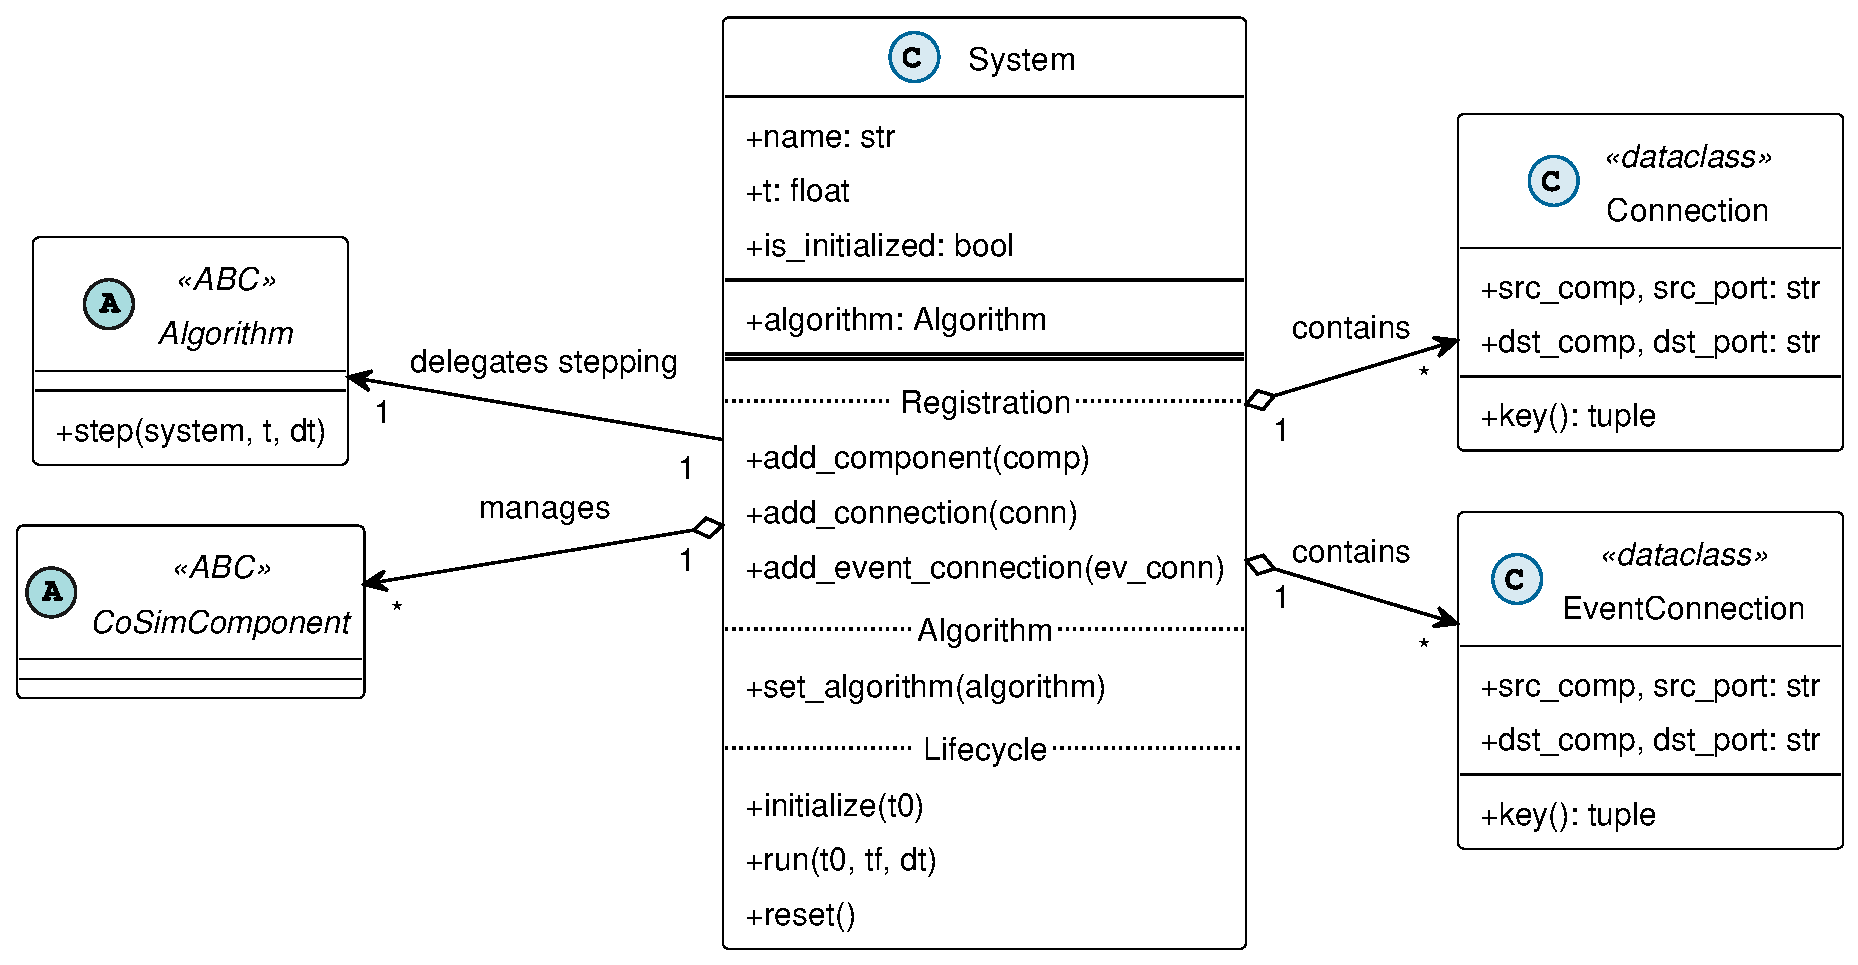
\includegraphics[width=0.85\textwidth]{diagrams/out/pdf/class/system/System.pdf}
    \caption{Class-level overview of the \texttt{System} abstraction in \syssimx. The diagram shows how the \texttt{System} manages components, stores signal and event connections, and delegates stepping to an \texttt{Algorithm}.}
    \label{fig:impl_system_class}
\end{figure}

%%%%%%%%%%%%%%%%%%%%%%%%%%%%%%%%%%%%%%%%%%%%%%%%%%%%%%
\subsection{Responsibilities and Stored State}

A \texttt{System} instance stores the structural definition of a co-simulation scenario.
This includes the registered components, signal connections, event connections, selected algorithm, and aggregated history.
It also tracks the current simulation time and the initialization state.
Derived metadata such as dependency graphs, algebraic loops, and execution order is introduced in Section~\ref{sec:impl_structural}.

%%%%%%%%%%%%%%%%%%%%%%%%%%%%%%%%%%%%%%%%%%%%%%%%%%%%%%
\subsection{Component Registration}

Components are registered with \texttt{add\_component()} before any connection can reference them.
Registration enforces that each component name is unique within the system and rejects additions after \texttt{initialize()} has been called, which keeps the structural analysis valid for the entire simulation run.
The component's history is registered with the system-level \texttt{SystemHistory} instance so that results from all components can be retrieved through a single call to \texttt{get\_history()} after the simulation.

%%%%%%%%%%%%%%%%%%%%%%%%%%%%%%%%%%%%%%%%%%%%%%%%%%%%%%
\subsection{Signal Connections}

A signal connection is represented by a immutable \texttt{Connection} object.
It stores the source component and output port together with the destination component and input port.
The object is frozen and hashable, so it can be used directly during duplicate checks and graph construction.

\paragraph{Validation.}
Signal connections are registered through \texttt{add\_connection()}.
Before a connection is stored, \texttt{\_validate\_connection()} checks that both components exist, both ports exist, the port specifications are compatible, and no duplicate connection is already registered.
The same validation also enforces single assignment.
A new connection is rejected if another connection already drives the same destination input.

\paragraph{Single Assignment.}
Each input port may be driven by at most one signal connection.
This invariant is enforced during connection registration.
The method \texttt{add\_connection()} rejects a new connection if another registered connection already targets the same destination component and input port.
This guarantees a unique source for every consumed input port.

%%%%%%%%%%%%%%%%%%%%%%%%%%%%%%%%%%%%%%%%%%%%%%%%%%%%%%
\subsection{Event Connections}

Hybrid scenarios use \texttt{EventConnection} to register a directed link from an event indicator of a source component to an event-handling target component.
The source port identifies the registered event indicator, and the destination port identifies the event input of the target that appears in the system graph.
The zero-crossing direction is not part of the connection.
It is defined once by the source component's event indicator and inherited by the generated event subscription.

The method \texttt{add\_event\_connection()} validates the connection, auto-subscribes the target, and updates the internal routing table from event source to target components.
The subscription is realized by appending a matching \texttt{Event} object to the target's \texttt{event\_subscriptions} list, which is the structure consumed by the hybrid algorithm of Section~\ref{sec:impl_hybrid}.
If a matching subscription is already present, it is not duplicated, so the same subscription can be expressed through manual registration or through \texttt{add\_event\_connection()} without conflicting entries on the target.
A duplicate event connection itself, however, is rejected at registration time.

%%%%%%%%%%%%%%%%%%%%%%%%%%%%%%%%%%%%%%%%%%%%%%%%%%%%%%
\subsection{Algorithm Selection}

The stepping algorithm is stored in the \texttt{algorithm} attribute and can be replaced through \texttt{set\_algorithm()}.
A \texttt{GaussSeidelAlgorithm} is installed at construction as a default that is appropriate for systems without state events.
At the start of \texttt{initialize()}, the system classifies the registered components into event sources, event listeners, and continuous-only components.
If any event sources are present, the algorithm is replaced by \texttt{HybridAlgorithm} irrespective of whether the user has set a different algorithm explicitly.
This ensures that the hybrid features of the framework are active whenever a component can produce state events and removes the need for the user to select the algorithm manually.

%%%%%%%%%%%%%%%%%%%%%%%%%%%%%%%%%%%%%%%%%%%%%%%%%%%%%%
\subsection{Lifecycle Orchestration}

Once all components and connections are registered, the system is driven through three phases.

\paragraph{Initialization.}
\texttt{initialize(t0)} first classifies the registered components and selects the hybrid algorithm when event sources are present.
It then prepares the component ports, computes direct-feedthrough metadata, and invokes the structural analysis of Section~\ref{sec:impl_structural}.
The resulting execution order is used to initialize the system generation by generation, as shown in Figure~\ref{fig:impl_system_initialization}.
For each generation, the system propagates upstream outputs, initializes the contained components, resolves local algebraic loops when needed, and performs a zero-step to publish outputs for downstream generations.
After initialization, the structural definition is fixed for the simulation run.

\begin{figure}[t]
  \centering
  \includegraphics[width=\linewidth]{diagrams/out/pdf/execution/System_Initialization.pdf}
  \caption[System initialization sequence.]{Sequence of operations executed by \texttt{System.initialize(t0)}.
    After classification, port preparation, and structural analysis, the system iterates over the execution order and, for each generation, propagates upstream outputs, initializes the contained components, resolves any algebraic loops, and performs a zero-step.
    The zero-step publishes direct-feedthrough outputs so that later generations are initialized with consistent input values.}
  \label{fig:impl_system_initialization}
\end{figure}

\paragraph{Run.}
\texttt{run(t0, tf, dt)} drives the coupled simulation by repeatedly delegating to the algorithm's \texttt{step()} method.
The stepping loop advances the time pointer in fixed macro steps of size \texttt{dt} and clamps the final step to the end time.
All orchestration details that depend on the chosen algorithm, such as input propagation between components, algebraic-loop iteration, and event localization, are owned by the algorithm (Section~\ref{sec:impl_algorithms}) and not by the \texttt{System} itself.

\paragraph{Reset.}
\texttt{reset()} releases the runtime state of the system without removing its structural definition.
It clears the aggregated history, resets all registered components through their own \texttt{reset()} hooks, and marks the system as not initialized.
The registered components, signal connections, event connections, and selected algorithm are retained, so the same scenario can be initialized and executed again without rebuilding the system configuration.

%%%%%%%%%%%%%%%%%%%%%%%%%%%%%%%%%%%%%%%%%%%%%%%%%%%%%%
\subsection{Verification}

The verification focuses on the registration contract of the \texttt{System}.
A valid registration must either extend the structural definition or be rejected before simulation state is changed.
The scenario uses lightweight mock components and checks signal connections, event connections, and lifecycle protection.
Table~\ref{tab:system_verification} summarizes the observed behavior.


\begin{table}[t]
  \centering
  \small
  \caption{Verification of the \texttt{System} registration contract.}
  \label{tab:system_verification}
  \begin{tabular}{p{3.2cm} p{6cm} p{6cm}}
    \toprule
    \textbf{Verified aspect} & \textbf{Minimal setup} & \textbf{Observed result} \\
    \midrule
    Signal connection registration
      & Three simple feedthrough components are registered.
        A valid connection from \texttt{A.y} to \texttt{C.u} is added.
        A second connection from \texttt{B.y} to the same input \texttt{C.u} is attempted.
      & The first connection is stored.
        The second connection is rejected with a \texttt{ValueError}.
        This confirms that each input port has a unique driver. \\
    \addlinespace

    Event connection registration
      & A hybrid source declares an event indicator.
        A hybrid listener declares a matching event input.
        An \texttt{EventConnection} links the source indicator to the listener input.
      & The target component receives exactly one matching event subscription.
        The subscription direction is inherited from the source event indicator.
        The connection itself only represents event routing. \\
    \addlinespace

    Lifecycle protection
      & The system is initialized after component and connection registration.
        A further component registration is attempted after initialization.
      & Initialization stores the system time and marks the system as initialized.
        Further component registration is rejected.
        The structural definition is therefore fixed for the simulation run. \\
    \bottomrule
  \end{tabular}
\end{table}

The scenario confirms that the registration contract is enforced uniformly across its three entry points.
The system rejects ambiguous or late structural changes before simulation starts, and event routing is configured through \texttt{EventConnection} while the event semantics remain owned by the source-side event indicator.
Structural-analysis properties are verified separately in Section~\ref{sec:impl_structural}.
%%%%%%%%%%%%%%%%%%%%%%%%%%%%%%%%%%%%%%%%%%%%%%%%%%%%%%%%%%%%%%%%
\section{Structural Analysis and Execution Ordering}
\label{sec:impl_structural}

This section describes the implementation of the structural analysis introduced in Section~\ref{sec:233_cosim_structural_analysis}.
The implementation realizes SR-10-02 and SR-10-03 under UR-10, and SR-11-02 under UR-11.
It derives persistent graph metadata from the registered components, signal connections, and direct-feedthrough information.
This metadata is later consumed by coupled initialization and by the master algorithms.

%%%%%%%%%%%%%%%%%%%%%%%%%%%%%%%%%%%%%%%%%%%%
\subsection{Inputs and Stored Metadata}
\label{sec:impl_structural_inputs}

Structural analysis is a pure function of information already registered with the \texttt{System}.
Its inputs are the registered components in \texttt{components}, the signal connections in \texttt{connections}, and the direct-feedthrough metadata each component exposes through \texttt{direct\_feedthrough} after feedthrough detection.
An auxiliary input is the set of \emph{active outputs}, that is, the output ports that are actually referenced by at least one outgoing connection.
This set is recomputed from the connection list and controls the active-output filter of Section~\ref{sec:impl_structural_graph}.

All results of the structural analysis are stored directly on the \texttt{System} instance so that the master algorithms and the initialization loop can read them without recomputation.
Table~\ref{tab:structural_metadata} lists the stored fields, the routine that produces them, and their purpose.
The attribute \texttt{\_dag} is called the \emph{zero-delay graph} throughout this section because it may contain cycles before algebraic-loop condensation.
It becomes acyclic only once each strongly connected component is collapsed into a single node during the computation of the execution order.

\begin{table}[!htbp]
  \centering
  \small
  \caption{Structural metadata stored on a \texttt{System} instance.
    All fields are populated during \texttt{initialize(t0)} and remain valid for the rest of the simulation run.}
  \label{tab:structural_metadata}
  \begin{tabular}{p{3.2cm} p{3.6cm} p{7.0cm}}
    \toprule
    \textbf{Attribute} & \textbf{Produced by} & \textbf{Purpose} \\
    \midrule
    \texttt{graph}
      & \texttt{build\_graphs()}
      & Full \texttt{MultiDiGraph} of all registered signal connections, including delayed ones. Used for visualization and for delayed-producer detection. \\
    \addlinespace
    \texttt{\_dag}
      & \texttt{build\_graphs()}
      & Zero-delay dependency graph restricted to connections whose destination input participates in active direct feedthrough. May contain cycles before condensation. \\
    \addlinespace
    \texttt{\_incoming\_by\_dst}
      & \texttt{build\_graphs()}
      & Incoming connections keyed by destination component. Used during input propagation. \\
    \addlinespace
    \texttt{\_input\_sources}
      & \texttt{build\_graphs()}
      & Mapping from destination component and port to the unique driving connection. Used by \texttt{\_set\_inputs\_for\_generation()}. \\
    \addlinespace
    \texttt{algebraic\_loops}
      & \texttt{build\_graphs()}
      & List of strongly connected components of the zero-delay graph with more than one node, plus one-component self-loops. Consumed by the IJCSA solver of Section~\ref{sec:impl_algebraic_loops}. \\
    \addlinespace
    \texttt{\_scc\_index}
      & \texttt{compute\_execution\_order()}
      & Mapping from component name to the condensation-node identifier it belongs to. \\
    \addlinespace
    \texttt{execution\_order}
      & \texttt{compute\_execution\_order()}
      & Generation-based schedule after condensation and delayed-producer post-processing. Each entry is a list of component names executed together. \\
    \addlinespace
    \texttt{execution\_idx}
      & \texttt{compute\_execution\_order()}
      & Mapping from component name to its generation index in \texttt{execution\_order}. \\
    \bottomrule
  \end{tabular}
\end{table}

%%%%%%%%%%%%%%%%%%%%%%%%%%%%%%%%%%%%%%%%%%%%
\subsection{Graph Construction}
\label{sec:impl_structural_graph}

Graph construction is performed by \texttt{build\_graphs()} and produces both the full connection graph and the zero-delay graph in a single pass over the registered connections.
It consists of four steps.
The first step clears any previously cached structural metadata so that a repeated call on the same system yields a well-defined result.
The second step adds every registered component as a node of both \texttt{graph} and \texttt{\_dag}, which guarantees that isolated components remain visible in the metadata even if they have no incoming or outgoing signal connections.
The third step collects the active-output set through \texttt{collect\_active\_outputs()}.
This set contains, for each component, those output ports that are referenced by at least one outgoing signal connection and is used as a filter during zero-delay edge insertion.

\paragraph{Full Connection Graph.}
The fourth step iterates over all signal connections.
Every connection is added to \texttt{graph} as an annotated multi-edge whose \texttt{src\_port} and \texttt{dst\_port} attributes identify the connected ports.
The same pass also populates the input-lookup maps \texttt{\_incoming\_by\_dst} and \texttt{\_input\_sources}.
Both maps are consumed later by \texttt{System.\_set\_inputs\_for\_generation()} to propagate upstream outputs into the input port states of the current generation.

\paragraph{Zero-Delay Graph and Active-Output Filter.}
Execution ordering only depends on instantaneous dependencies, so \texttt{\_dag} is built from a strict subset of the connections that enter \texttt{graph}.
A signal connection from component $A$ to component $B$ is added to \texttt{\_dag} if and only if the connected destination port of $B$ participates in the direct feedthrough of at least one \emph{active} output of $B$.
This condition is evaluated against the \texttt{direct\_feedthrough} mapping of component $B$, which is produced during feedthrough detection (Section~\ref{sec:impl_component_interface}) and lists, for each output port, the set of input ports on which it depends algebraically.
The active-output restriction is what distinguishes the \syssimx{} zero-delay graph from the purely conceptual version shown in Section~\ref{sec:233_cosim_structural_analysis}.
A feedthrough path through component $B$ only contributes an ordering constraint if its output is actually consumed by another component, because an unused output cannot influence the coupled dynamics.
The filter therefore removes ordering constraints that would otherwise be imposed by sink-like outputs without changing the simulation semantics.

%%%%%%%%%%%%%%%%%%%%%%%%%%%%%%%%%%%%%%%%%%%%
\subsection{Algebraic Loop Detection}
\label{sec:impl_structural_loops}

Once the zero-delay graph has been assembled, \texttt{build\_graphs()} identifies the subsets of components that participate in an instantaneous cyclic dependency.
Section~\ref{sec:233_cosim_algebraic_loops} has already established that each such subset corresponds to a strongly connected component of the zero-delay graph.
This implementation reuses that result directly through \texttt{networkx.strongly\_connected\_components()}, which returns every maximal strongly connected subset of \texttt{\_dag}.

\paragraph{Multi-Component Loops.}
Any strongly connected component with more than one node is stored as an algebraic loop in the attribute \texttt{algebraic\_loops}.
Each entry is a list of component names that collectively form one loop block.
The ordering inside a block is not semantically relevant at this stage, because the IJCSA solver of Section~\ref{sec:impl_algebraic_loops} treats the block as an unordered set of unknowns and equations.

\paragraph{Single-Component Self-Loops.}
A one-component algebraic loop arises when an output of a single component depends instantaneously on one of its own inputs through an outer connection that feeds the component's output back into its own input.
Such a configuration produces a self-loop in \texttt{\_dag}.
The first pass over the strongly connected components does not recognize this case because a single node always forms a strongly connected component of size one.
A second explicit pass iterates over all nodes, checks whether the node carries a self-loop edge in \texttt{\_dag}, and, if so, appends the corresponding singleton list to \texttt{algebraic\_loops}.
From the perspective of the master algorithm a self-loop is a regular loop block with one participant.
This unified representation realizes SR-11-02 and allows the iterative solver to apply the same IJCSA iteration scheme to multi-component and one-component loops without special casing.

\paragraph{Consumers of the Loop Information.}
Two later stages of the pipeline consume \texttt{algebraic\_loops}.
The condensation step of Section~\ref{sec:impl_structural_condensation} uses the strongly connected components of \texttt{\_dag} to collapse each loop into a single condensed node before the topological generations are computed.
The initialization loop of \texttt{System.initialize(t0)} and every master algorithm subsequently iterate over \texttt{algebraic\_loops} for each generation and hand loops whose members are contained entirely in the current generation to the IJCSA solver.
The detection pass described here is therefore performed once during structural analysis and its result remains valid for the rest of the simulation run.

%%%%%%%%%%%%%%%%%%%%%%%%%%%%%%%%%%%%%%%%%%%%
\subsection{Condensation and Execution Order}
\label{sec:impl_structural_condensation}

The zero-delay graph may contain directed cycles, so a topological sort cannot be applied to it directly.
Section~\ref{sec:233_cosim_structural_analysis} has shown that collapsing every strongly connected component into a single node yields the condensed graph, which is acyclic by construction.
The routine \texttt{compute\_execution\_order()} implements this idea on \texttt{\_dag} and then derives the generation-based schedule that the master algorithms consume.

\paragraph{Condensation.}
The condensation is obtained through \texttt{networkx.condensation()}.
The result is a directed acyclic graph whose nodes are integer identifiers of the strongly connected components of \texttt{\_dag} and whose edges reflect the inter-component dependencies that survive the collapse.
The returned mapping from original component names to condensation identifiers is inverted once and stored in two auxiliary structures.
The mapping \texttt{\_scc\_index} records, for each component, the identifier of the strongly connected component it belongs to and is used during initialization and during loop resolution to locate a component's loop block.
A second local dictionary stores the reverse direction, that is, the sorted list of component names contained in each condensation node.
It is only needed during execution-order construction and is discarded afterwards.

\paragraph{Topological Generations.}
The acyclic condensed graph is passed to \texttt{networkx.topological\_generations()}, which returns a sequence of sets of condensation nodes such that all dependencies of a set have already been satisfied by earlier sets.
Each set is one \emph{generation} in the sense of Section~\ref{sec:233_cosim_structural_analysis}.
\syssimx{} expands every condensation identifier back to its constituent component names and stores the resulting generations as a list of lists in \texttt{execution\_order}.
The component names inside a generation are sorted alphabetically so that the schedule is deterministic and independent of the registration order.
A generation therefore contains either a set of mutually independent components, which can in principle be advanced in parallel, or the members of one algebraic loop, which must be resolved locally before the generation is considered advanced.

\paragraph{Index Lookup.}
The auxiliary dictionary \texttt{execution\_idx} is built in the same pass and maps every component name to the zero-based index of the generation that owns it.
This index is queried by the master algorithms when they need to decide whether a given component is upstream of another without traversing \texttt{\_dag}.
Because both \texttt{execution\_order} and \texttt{execution\_idx} are rebuilt in every invocation, a repeated call on the same system reflects the current state of connections and direct-feedthrough metadata.

\paragraph{Post-Processing.}
The schedule produced by the topological generations is the structurally correct order of execution, but it does not yet account for the \syssimx{}-specific placement of delayed producers.
That adjustment is described in Section~\ref{sec:impl_structural_delayed} and is applied as the final step of \texttt{compute\_execution\_order()} before the routine returns.

%%%%%%%%%%%%%%%%%%%%%%%%%%%%%%%%%%%%%%%%%%%%
\subsection{Delayed Producer Post-Processing}
\label{sec:impl_structural_delayed}

The condensation-based schedule of Section~\ref{sec:impl_structural_condensation} captures every ordering constraint that follows from instantaneous dependencies.
Some components, however, have no zero-delay edges at all and yet reach the strongly coupled part of the system through purely delayed connections.
A typical example is an actuator component whose output influences the plant dynamics only through a downstream integrator.
The topological generations treat such components as isolated and place them arbitrarily early in the schedule.
This is correct with respect to zero-delay dependencies, but it advances the component before the loop block that it ultimately feeds has produced a consistent output for the current step.
\syssimx{} therefore applies a post-processing step that relocates those components to the end of the schedule.
The step is a scheduling choice of the framework and not a general property of co-simulation theory.

\paragraph{Delayed-Producer Criterion.}
A component is classified as a delayed producer if two conditions are satisfied simultaneously.
First, it must have neither incoming nor outgoing edges in the zero-delay graph \texttt{\_dag}, so it contributes no algebraic feedthrough to the coupled dynamics.
Second, it must still reach at least one component with zero-delay structure through the full connection graph \texttt{graph}, which means that its outputs influence the coupled part of the system through a sequence that contains at least one delayed edge.
The predicate \texttt{is\_delayed\_producer()} evaluates both conditions and short-circuits as soon as a reachable zero-delay node is found.

\paragraph{Relocation Step.}
The routine \texttt{move\_delayed\_producers\_to\_last\_generation()} collects all components for which the predicate is true, removes them from their original generations, and appends them as an additional final generation that is sorted alphabetically for determinism.
Empty generations that may arise from the removal are dropped so the schedule stays compact.
The auxiliary index \texttt{execution\_idx} is rebuilt after the relocation so that every component's generation index remains consistent with \texttt{execution\_order}.
If no component satisfies the predicate, the schedule is left unchanged, which is the common case for scenarios without delayed producers.


\subsection{Use by Initialization and Master Algorithms}
\label{sec:impl_structural_use}

The metadata produced in the preceding subsections is computed once at the start of \texttt{System.initialize(t0)} and then consumed read-only for the rest of the simulation run.
The initialization loop of Section~\ref{sec:impl_system} iterates over \texttt{execution\_order} generation by generation, uses \texttt{\_input\_sources} to propagate upstream outputs into the current generation, and hands every entry of \texttt{algebraic\_loops} whose members are contained entirely in that generation to the IJCSA solver of Section~\ref{sec:impl_algebraic_loops}.
The Jacobi, Gauss--Seidel, and Hybrid algorithms of Section~\ref{sec:impl_algorithms} reuse the same metadata during stepping and additionally query \texttt{execution\_idx} when they need to compare the positions of two components in the schedule.
The structural analysis is therefore a one-shot preprocessing stage whose output defines a fixed orchestration contract between \texttt{System} and the master algorithms for the remainder of the run.

\subsection{Verification}

%%%%%%%%%%%%%%%%%%%%%%%%%%%%%%%%%%%%%%%%%%%%%%%%%%%%%%%%%%%%%%%%
\section{Algebraic Loop Resolution}
\label{sec:impl_algebraic_loops}

The algebraic-loop implementation realizes \ref{req:SR-11-03} under \ref{req:UR-11}.
It uses the SCC-local loop blocks detected by the structural analysis of Section~\ref{sec:impl_structural}.
The theoretical basis is introduced in Section~\ref{sec:235_cosim_algebraic_loops}.
When a master algorithm reaches a loop generation, \syssimx{} computes mutually consistent interface values before any component in the loop block advances its state.
The local solver \pyfn{solve\_algebraic\_scc\_ijcsa()} performs this correction for one strongly connected component.
The global \texttt{IJCSAAlgorithm} solves the complete zero-delay interface and is described in Section~\ref{sec:impl_algorithms}.

%%%%%%%%%%%%%%%%%%%%%%%%%%%%%%%%%%%%%%%%%%%%
\subsection{Scope and Local Interface Data}
\label{sec:impl_algebraic_loops_scope}

The local solver operates on a single \ac{SCC} $\mathcal{L}$ and reuses the structural metadata stored on the \texttt{System} instance.
From the zero-delay connections incident to $\mathcal{L}$ it derives four artifacts that together define the local interface problem.
The first artifact is the vector of interface unknowns
\begin{equation}
  U_{\mathcal{L}} = \bigl(u_1,\ldots,u_n\bigr)^\top,
\end{equation}
which collects every destination input port of a zero-delay connection whose source and destination components both belong to $\mathcal{L}$.
The second artifact is a map \pyfn{driver\_for\_input} that resolves each entry of $U_{\mathcal{L}}$ to the source output port that drives it inside $\mathcal{L}$.
The third artifact is the set of internal connections, which are the zero-delay edges with both endpoints in $\mathcal{L}$ and which couple the unknowns through component outputs.
The fourth artifact is the set of external incoming connections, which are zero-delay edges that enter $\mathcal{L}$ from components in earlier generations.
Their driver outputs are read once at the current communication point and kept fixed during the local solve, so they contribute known right-hand-side values rather than additional unknowns.

%%%%%%%%%%%%%%%%%%%%%%%%%%%%%%%%%%%%%%%%%%%%
\subsection{Residual Evaluation}
\label{sec:impl_algebraic_loops_residual}

For a trial vector $U_{\mathcal{L}}$, the solver assembles temporary inputs for every component in $\mathcal{L}$.
These inputs contain the trial values and the fixed external values.
The solver then calls \pyfn{evaluate\_outputs(inputs)} on each component.

Routing the returned outputs through \pyfn{driver\_for\_input} yields the induced interface vector $\widehat{U}_{\mathcal{L}}(U_{\mathcal{L}})$.
The residual is
\begin{equation}
  \mathcal{R}_{\mathcal{L}}(U_{\mathcal{L}}) = U_{\mathcal{L}} - \widehat{U}_{\mathcal{L}}(U_{\mathcal{L}}),
\end{equation}
which matches the fixed-point form of Section~\ref{sec:235_cosim_algebraic_loops} restricted to $\mathcal{L}$.
A consistent loop state is reached when $\|\mathcal{R}_{\mathcal{L}}\|_2$ falls below the solver tolerance.
Because \pyfn{evaluate\_outputs()} does not advance component state, the residual can be sampled at several trial vectors within one macro step.

%%%%%%%%%%%%%%%%%%%%%%%%%%%%%%%%%%%%%%%%%%%%
\subsection{Newton Iteration and Commit}
\label{sec:impl_algebraic_loops_newton}

The iteration starts from the values currently stored in the destination input ports of $\mathcal{L}$.
These values are the most recent consistent inputs from the previous macro step.
Each iteration approximates the interface Jacobian column-wise by forward finite differences,
\begin{equation}
  J^{(m)}_{:,j} \approx
  \frac{
    \mathcal{R}_{\mathcal{L}}\!\bigl(U_{\mathcal{L}}^{(m)} + \varepsilon e_j\bigr)
    - \mathcal{R}_{\mathcal{L}}\!\bigl(U_{\mathcal{L}}^{(m)}\bigr)
  }{\varepsilon},
  \qquad \varepsilon = 10^{-6},
\end{equation}
and applies the standard Newton update $U_{\mathcal{L}}^{(m+1)} = U_{\mathcal{L}}^{(m)} - \bigl(J^{(m)}\bigr)^{-1}\mathcal{R}_{\mathcal{L}}(U_{\mathcal{L}}^{(m)})$.

The loop terminates when $\|\mathcal{R}_{\mathcal{L}}\|_2<\texttt{tol}$.
If the Jacobian is singular or the residual fails to converge within \texttt{max\_iter} iterations, the solver aborts the current macro step with a runtime error rather than committing inconsistent inputs.
The Jacobian becomes singular when the loop-gain eigenvalue approaches one, for example for an identity feedback $y=u$ or a unit-gain cycle.
Finite-difference noise at discontinuities can produce the same condition numerically.

After convergence the solver writes the solved entries of $U_{\mathcal{L}}$ back to the corresponding destination input ports through \pyfn{inputs[dst].set(value, t)}, so the loop inputs are mutually consistent at the current communication point while the component states are still unchanged.
The active master algorithm then performs the subsequent macro step on the basis of these committed values.

%%%%%%%%%%%%%%%%%%%%%%%%%%%%%%%%%%%%%%%%%%%%
\subsection{Verification Scenario}
\label{sec:impl_algebraic_loops_verification}

The verification scenario of Figure~\ref{fig:algebraic_loop_verification} consists of a constant source, two subtractors, and one integrator.
The labels on the ports define the notation used below.

\begin{figure}[H]
  \centering
  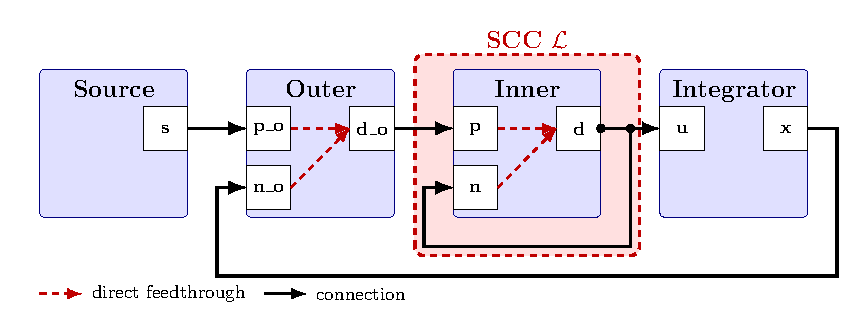
\includegraphics[width=0.9\linewidth]{figures/5_implementation/algebraic_loop/algebraic_loop_verification.pdf}
  \caption{Verification scenario for algebraic loops. The dashed red rectangle marks the SCC node set $\mathcal{L}=\{\texttt{Inner}\}$. Wire routing is purely visual and does not indicate SCC membership.}
  \label{fig:algebraic_loop_verification}
\end{figure}

The \texttt{Source} emits $s=1$.
The two subtractors \texttt{Inner} and \texttt{Outer} are direct-feedthrough components with output equation $d_o=p_o-n_o$ and $d=p-n$ respectively.
The \texttt{Integrator} advances $\dot{x}=u$ with $x(0)=0$ and has no feedthrough.
Five connections close the topology.
The source drives the positive input of \texttt{Outer}.
The output of \texttt{Outer} drives the positive input of \texttt{Inner}.
The output of \texttt{Inner} drives the integrator input and is also fed back to its own negative input.
The integrator output drives the negative input of \texttt{Outer}.
This last connection is delayed because the integrator has no direct feedthrough from $u$ to $x$.

The self-connection $d\to n$ is the only zero-delay cycle, so the structural analysis stores a single SCC $\mathcal{L}=\{\texttt{Inner}\}$.
For the local solve, $n$ is the only interface unknown and the edge $d_o\to p$ appears as the one external incoming connection held fixed at the current communication point.
At $t=0$ the integrator output is zero, so the external value reduces to $p=s-x=1$.
The local problem collapses to the scalar fixed-point equation $n=p-n$ with analytical solution $n=d=\tfrac{1}{2}p=0.5$.

\begin{listing}[ht]
  \begin{lstlisting}[
    basicstyle=\ttfamily\footnotesize,
    frame=single,
    backgroundcolor=\color{black!3},
    breaklines=true,
    columns=fullflexible,
    xleftmargin=0pt
]
Solving algebraic SCC ['Inner']:
  Interface inputs:                [('Inner', 'neg')]
  Internal zero-delay connections: [('Inner', 'diff', 'Inner', 'neg')]
  External zero-delay inputs:      [('Outer', 'diff', 'Inner', 'pos')]
  Initial guess for Inner.neg = -0.001
Starting IJCSA iterations:
  Iteration 0: u = [-0.001]
    Residual for Inner.neg: -1.0019999999999998
    Jacobian J = [[2.]]
    Correction du = [0.501]
  Iteration 1: u = [0.5]
    Residual for Inner.neg: 8.243e-11
  Converged in 1 iterations.
Committed solved input Inner.neg = 0.5000000000412155
\end{lstlisting}
  \caption{IJCSA solver trace for the algebraic-loop verification scenario.
    The local solver identifies the scalar interface problem and converges to the analytical solution in one Newton step.}
  \label{lst:ijcsa_verification_log}
\end{listing}

Listing~\ref{lst:ijcsa_verification_log} confirms the expected local interface problem.
The solver identifies one interface unknown, one internal self-connection, and one external incoming zero-delay input.
Starting from the initial guess, it converges to $n=0.5$ in one Newton step and commits the value before the macro step.
This agrees with the analytical solution and verifies the SCC-local loop solve.
%%%%%%%%%%%%%%%%%%%%%%%%%%%%%%%%%%%%%%%%%%%%%%%%%%%%%%%%%%%%%%%%
\section{Master Algorithms}
\label{sec:impl_algorithms}

This section addresses SR-11-03 (numerical treatment of algebraic loops) and explains how \syssimx{} realizes the master algorithms introduced in Section~\ref{sec:234_cosim_execution_strategies}.
The structural analysis of Section~\ref{sec:impl_structural} already provides the execution generations and the detected algebraic loops.
Section~\ref{sec:impl_algebraic_loops} already defined the SCC-local loop solver.
The present section therefore focuses on the orchestration of one macro step by the concrete classes \texttt{JacobiAlgorithm}, \texttt{GaussSeidelAlgorithm}, and \texttt{IJCSAAlgorithm}.
Hybrid event handling is excluded here and is explained in Section~\ref{sec:impl_hybrid}.

%%%%%%%%%%%%%%%%%%%%%%%%%%%%%%%%%%%%%%
\subsection{Scope and Shared Metadata}
\label{sec:impl_algorithms_scope}

All master algorithms consume the same execution metadata stored on the \texttt{System} instance during initialization.
The list \pyfn{execution\_order} defines the generation order, \pyfn{algebraic\_loops} identifies the loop blocks, and \pyfn{\_set\_inputs\_for\_generation()} propagates signal values to the destination input ports of one generation.
The Jacobi and Gauss--Seidel algorithms reuse the SCC-local solver of Section~\ref{sec:impl_algebraic_loops}.
The global \pyfn{IJCSAAlgorithm} replaces this local treatment by one global interface solve before the macro steps are executed.

Across all three algorithms, one macro step consists of two tasks.
First, the interface values at the current communication point are propagated and, if required, corrected so that the zero-delay couplings are consistent.
Second, the components advance from $t$ to $t+\Delta t$ by calling \texttt{do\_step(t, dt)}.
The algorithms differ only in how these tasks are ordered across the generations and in whether the interface correction is carried out locally per loop block or globally for the complete system.

Figure~\ref{fig:impl_algorithms_jacobi_gs} summarizes the implementation-level execution flow of the two explicit continuous master algorithms.

\begin{figure}[!htbp]
    \vspace{-1em}
    \centering
    \begin{subfigure}[t]{0.48\linewidth}
        \centering
        \begin{minipage}[t][9.8cm][t]{\linewidth}
            \vspace{0pt}
            \centering
            \includegraphics[width=\linewidth]{diagrams/out/pdf/execution/Jacobi_Algorithm.pdf}
        \end{minipage}
        \caption{Jacobi execution. All generations are prepared first. The component steps are executed only afterwards.}
        \label{fig:impl_algorithms_jacobi}
    \end{subfigure}
    \hfill
    \begin{subfigure}[t]{0.48\linewidth}
        \centering
        \begin{minipage}[t][9.8cm][t]{\linewidth}
            \vspace{0pt}
            \centering
            \includegraphics[width=\linewidth]{diagrams/out/pdf/execution/Gauss_Seidel_Algorithm.pdf}
        \end{minipage}
        \caption{Gauss--Seidel execution. Each generation is prepared and stepped immediately before the next one is processed.}
        \label{fig:impl_algorithms_gs}
    \end{subfigure}
    \caption{Implementation-level execution diagrams of the explicit continuous master algorithms.}
    \label{fig:impl_algorithms_jacobi_gs}
    \vspace{-1em}
\end{figure}

%%%%%%%%%%%%%%%%%%%%%%%%%%%%%%%%%%%%%%
\subsection{Jacobi Algorithm}
\label{sec:impl_algorithms_jacobi}

The class \texttt{JacobiAlgorithm} realizes the explicit non-iterative scheme of Section~\ref{sec:234_cosim_execution_strategies} by structuring one macro step in two phases over \texttt{execution\_order}.
In the first phase, the algorithm iterates through the generations.
For each one, it calls \pyfn{\_set\_inputs\_for\_generation(gen, t)} to stage the interface values at the current communication point.
If the generation contains algebraic loops, it then invokes \pyfn{solve\_algebraic\_scc\_ijcsa(system, loop, t)}.
In the second phase, the algorithm iterates through the generations a second time.
Every component of each generation is advanced by one step through \texttt{do\_step(t, dt)} with the interface values frozen at $t$.
Because no component advances before all interface values have been staged, components in later generations still read the output values produced at the previous communication point.
This is how the Jacobi property works at the implementation level.
All simulation units use the same communication-point snapshot.
The current implementation preserves this semantics through a serial loop over the generations, so the second phase would admit parallel execution of the component steps, but \syssimx{} does not yet exploit this.

%%%%%%%%%%%%%%%%%%%%%%%%%%%%%%%%%%%%%%

\subsection{Gauss--Seidel Algorithm}
\label{sec:impl_algorithms_gs}

The class \texttt{GaussSeidelAlgorithm} collapses the two phases of the Jacobi implementation into a single pass over \texttt{execution\_order}.
For each generation, the algorithm first stages the interface values through \pyfn{\_set\_inputs\_for\_generation(gen, t)}.
It then solves every loop block contained in that generation through \pyfn{solve\_algebraic\_scc\_ijcsa(system, loop, t)}.
The execution of \texttt{do\_step(t, dt)} moves every component of the generation to $t+\Delta t$.
The output ports of the components in earlier generations therefore already hold the values at $t+\Delta t$ when the inputs of a later generation are staged.
A call of \pyfn{\_set\_inputs\_for\_generation()} on the next generation propagates these fresh values into the destination ports.
This within-step visibility of updated outputs is the only algorithmic difference to the Jacobi implementation.
The local SCC solver, the input-staging routine, and the structural metadata on \texttt{System} are reused unchanged, which is why the two classes share the orchestration skeleton of Section~\ref{sec:impl_algorithms_scope} and differ only in where the \texttt{do\_step(t, dt)} call is placed relative to the generation loop.
The sequential per-generation ordering also implies that the Gauss--Seidel algorithm does not exploit the parallelism that the Jacobi second phase would admit in principle.

%%%%%%%%%%%%%%%%%%%%%%%%%%%%%%%%%%%%%%
%%%%%%%%%%%%%%%%%%%%%%%%%%%%%%%%%%%%%%
\subsection{Global IJCSA Algorithm}
\label{sec:impl_algorithms_ijcsa}

The class \texttt{IJCSAAlgorithm} provides a global counterpart to the SCC-local solver of Section~\ref{sec:impl_algebraic_loops}.
It implements the original Sicklinger formulation~\cite{sicklinger_interface_2014}, which treats the full set of zero-delay interface unknowns of the scenario as one coupled Newton system.

Its \texttt{step()} method runs in two phases.
The first phase calls \pyfn{solve\_global\_interface\_ijcsa(system, t)}.
This routine uses \pyfn{collect\_global\_interface\_unknowns()} to build the global unknown vector and the driver map.
A Newton iteration is then applied to the residual $\mathcal{R}(U)=U-\widehat{U}(U)$ with frozen component states, as in the local solver.
A damped-gradient fallback stabilizes the update when the Jacobian is singular.
After convergence, the solved interface values are written to the destination input ports.
In the second phase, \texttt{step()} traverses \texttt{execution\_order} and calls \texttt{do\_step(t, dt)} on every component.

Several elements of the original Sicklinger formulation are deliberately omitted in \syssimx{}.
The constraint operator is restricted to the signal-assignment form $U=\widehat{U}(U)$.
A general nonlinear interface constraint $L(U,Y)=0$ is not supported.
The inner evaluation reuses the side-effect-free \pyfn{evaluate\_outputs(inputs)} contract and keeps component states frozen at $t$.
Trial macro steps with rollback are therefore not required.
The interface Jacobian is always assembled by finite differences.
Directional derivatives exposed by the simulation units are not requested even when available.
Input extrapolation between communication points and an explicit relaxation factor are also absent.
The fixed point is reached with unit step length or with the damped-gradient fallback.

The global solve is mathematically redundant when the zero-delay SCCs are disjoint.
In that case its block-diagonal Jacobian is equivalent to running the local solver of Section~\ref{sec:impl_algebraic_loops} once per SCC, and the two variants produce the same fixed point in the same number of Newton iterations.
\texttt{IJCSAAlgorithm} is therefore included mainly for completeness and as a reference implementation of the original Sicklinger scheme.
The default orchestration path is \texttt{JacobiAlgorithm} or \texttt{GaussSeidelAlgorithm}, which invoke the local solver on demand and avoid assembling one large interface system for every macro step.

%%%%%%%%%%%%%%%%%%%%%%%%%%%%%%%%%%%%%%
\subsection{Verification}
\label{sec:impl_algorithms_verification}

Verification of the three master algorithms uses a small feedback scenario which combines a constant source, a gain block, a subtractor, and an integrator.
The only delayed edge is the one entering the integrator, so the zero-delay graph is acyclic and the structural analysis produces three generations without any SCC.
Figure~\ref{fig:impl_algorithms_verification_system} shows the resulting topology.

\begin{figure}[!htbp]
    \centering
    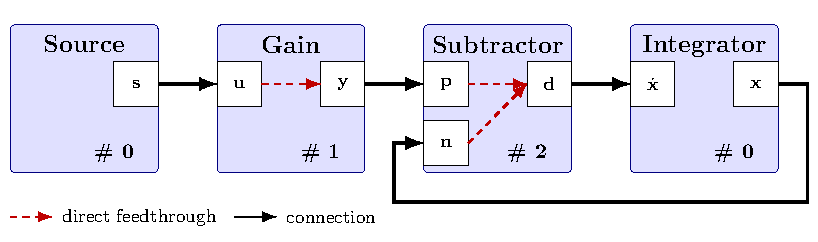
\includegraphics[width=0.85\linewidth]{figures/5_implementation/master_algorithms/master_algorithm_verification.pdf}
    \caption{Topology of the verification scenario. Solid black arrows are port-to-port connections. Dashed red arrows are internal direct-feedthrough relations. The generation index is shown in the lower-right corner of each component. Because the Integrator has no direct feedthrough from $\dot{x}$ to $x$, the inbound edge $\texttt{Subtractor.d} \to \texttt{Integrator.}\dot{x}$ is delayed. This is why the Integrator shares generation~$0$ with the Source and the zero-delay graph remains acyclic.}
    \label{fig:impl_algorithms_verification_system}
\end{figure}

The continuous dynamics reduce to the scalar ODE $\dot{y}=k\,r-y$ with $y(0)=0$.
Its analytical solution
\begin{equation}
    y(t) = k\,r\,\bigl(1-e^{-t}\bigr)
\end{equation}
serves as the reference.

Figure~\ref{fig:impl_algorithms_verification} compares all three algorithms against this reference for four macro step sizes with $k=2$ and $r=1$.

\begin{figure}[t]
    \vspace{-1ex}
    \centering
    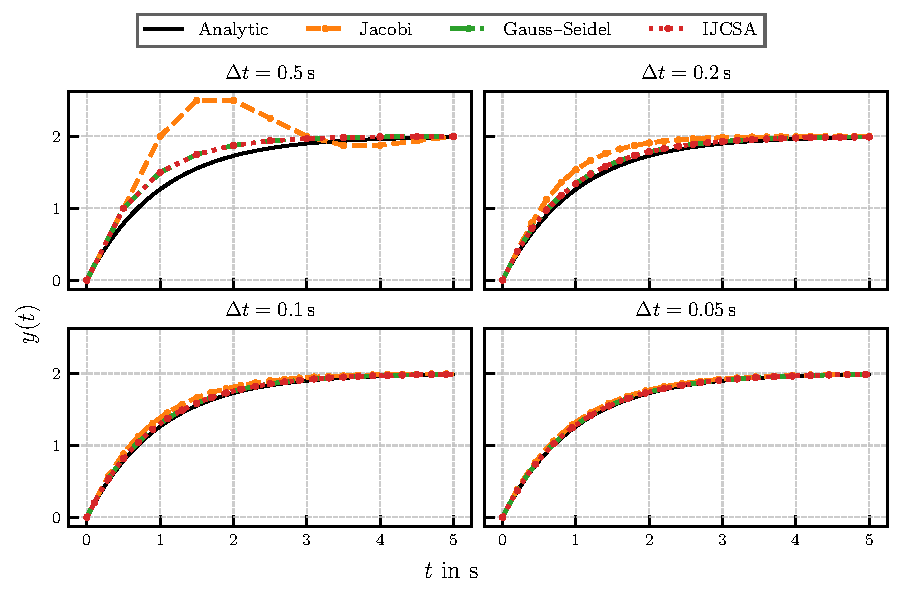
\includegraphics[width=0.9\linewidth]{figures/5_implementation/master_algorithms/algorithm_comparison.pdf}
    \caption{Jacobi, Gauss--Seidel, and Global IJCSA orchestration on a feedback scenario with direct feedthrough and one delayed edge into the integrator. The analytical solution $y(t)=kr(1-e^{-t})$ with $k=2$ and $r=1$ is shown in black. At $\Delta t=0.5\,$s the Jacobi trace overshoots the reference. The Gauss--Seidel and Global IJCSA traces stay close and overlap. All three traces converge to the analytical solution as $\Delta t$ is reduced.}
    \label{fig:impl_algorithms_verification}
\end{figure}

At $\Delta t = 0.5\,$s the Jacobi trace overshoots the analytical solution, while the Gauss--Seidel trace stays close to it.
The overshoot is a direct consequence of the two-phase structure of \texttt{JacobiAlgorithm}.
Components in later generations read output values from the previous communication point, so the feedback through the integrator reaches the subtractor with one macro-step delay.
The Gauss--Seidel pass propagates the updated subtractor output within the same macro step and therefore tracks the reference more closely.
The \texttt{IJCSAAlgorithm} trace overlaps the Gauss--Seidel trace in this scenario.
This is expected because the zero-delay graph is acyclic.
The global solve still contains the zero-delay interface inputs of the Gain and Subtractor components, but it does not resolve an algebraic loop.
After this consistency step, the algorithm advances the generations sequentially.
Its behavior therefore matches the Gauss--Seidel traversal for this example.
All three traces approach the analytical solution as the macro step size is reduced.
This verifies the expected orchestration behavior of the three master algorithms.

The scenario does not exercise algebraic-loop resolution because its zero-delay graph is acyclic.
The SCC-local Newton solve is verified separately in Section~\ref{sec:impl_algebraic_loops}.



%%%%%%%%%%%%%%%%%%%%%%%%%%%%%%%%%%%%%%%%%%%%%%%%%%%%%%%%%%%%%%%%
\section{Hybrid Co-Simulation Algorithm}
\label{sec:impl_hybrid}

The previous sections described the master algorithms and the structural metadata used during macro-step execution.
This section extends that implementation to hybrid co-simulation and realizes the concepts introduced in Section~\ref{sec:236_cosim_hybrid}.
It addresses SR-10-04 under UR-10 in Table~\ref{tab:req_simulation}, which requires system-level detection, localization, and propagation of discrete events across coupled subsystem models.
The hybrid orchestration is implemented as \texttt{HybridAlgorithm} and reuses \texttt{GaussSeidelAlgorithm} as the continuous algorithm, between events.
It also relies on the hybrid component hooks and event connections introduced in Sections~\ref{sec:impl_component_interface} and~\ref{sec:impl_system}.

%%%%%%%%%%%%%%%%%%%%%%%%%%%%%%%%%%%%%%%%%%%%%%%%%%%%%%
\subsection{Scope and Component Contract}
\label{sec:impl_hybrid_scope}

Hybrid execution is activated during \texttt{System.initialize(t0)}.
The system classifies the registered components into event sources, event listeners, and continuous-only components.
If at least one event source is present, the selected algorithm is replaced by \texttt{HybridAlgorithm}.
Otherwise, the continuous execution path remains unchanged.

A component becomes an event source by registering an indicator with \pyfn{add\_event\_indicator()}.
The resulting \texttt{EventIndicator} stores the scalar indicator function and the crossing direction.
Rollback support is required because event detection and localization use trial steps inside a macro step.
This requirement is enforced through \texttt{supports\_rollback} when the indicator is registered.
A component becomes an event listener when an \texttt{EventConnection} subscribes it to an event produced by another component.

Event times are stored as \texttt{DenseTime} objects.
Each object combines the physical time $t$ with a microstep index $\nu$.
This allows the algorithm to order cascaded events that occur at the same physical time.

Table~\ref{tab:hybrid_component_contract} summarizes the hybrid-specific operations used by \texttt{HybridAlgorithm}.
The general component interface is described in Section~\ref{sec:impl_component_interface}.

\begin{table}[htbp]
  \centering
  \caption{Hybrid component operations used by \texttt{HybridAlgorithm}.}
  \label{tab:hybrid_component_contract}
  \begin{tabular}{lp{10cm}}
    \toprule
    \textbf{Operation} & \textbf{Role in hybrid execution} \\
    \midrule
    \texttt{evaluate\_event\_indicators()} & Returns the current indicator values \\
    \texttt{detect\_event\_crossings()} & Detects crossings between two indicator states \\
    \texttt{snapshot\_state()} & Captures the rollback state before a trial step \\
    \texttt{restore\_state()} & Restores the component after trial stepping or bisection \\
    \texttt{handle\_event()} & Applies event-driven state updates \\
    \texttt{report\_internal\_event()} & Reports optional event brackets from internal micro-stepping \\
    \bottomrule
  \end{tabular}
\end{table}

Event routing is stored on the \texttt{System}.
During \pyfn{add\_event\_connection()}, each \pyfn{EventConnection} adds one source-event to listener mapping to \pyfn{\_event\_targets\_by\_source}.
The hybrid algorithm queries this mapping when localized events are dispatched.

%%%%%%%%%%%%%%%%%%%%%%%%%%%%%%%%%%%%%%%%%%%%%%%%%%%%%%
\subsection{Hybrid Macro-Step Sequence}
\label{sec:impl_hybrid_macro_step}

The entry point of the hybrid algorithm is \texttt{step(system, t, dt)}.
The method advances the system from the current communication time $t$ to $t + \Delta t$ and stores the interval boundaries as \texttt{t\_left} and \texttt{t\_right}.
An outer while loop iterates over \texttt{t\_left} so that one invocation of \texttt{step()} may internally resolve several events at different times in the interval.
Figure~\ref{fig:impl_hybrid_macro_step} summarizes the five phases of one outer iteration.

\begin{figure}[t]
    \centering
    \includegraphics[width=0.85\linewidth]{diagrams/out/pdf/execution/hybrid/Hybrid_Step.pdf}
    \caption{Implementation-level macro-step orchestration of the hybrid co-simulation algorithm.
    Each interval starts with input preparation and trial event detection.
    If no crossing is found, the remaining interval is advanced by the Gauss--Seidel path.
    If a crossing is found, the event time is localized, the system is advanced to that time, and event handling is iterated in superdense time until no further cascaded event remains.}
    \label{fig:impl_hybrid_macro_step}
\end{figure}

At each new value of \texttt{t\_left}, \texttt{\_prepare\_inputs()} propagates the current signal values generation by generation.
If a generation contains an algebraic loop, the local SCC solver from Section~\ref{sec:impl_algebraic_loops} is applied before event detection continues.
The algorithm then performs the trial-step-based detection described in Section~\ref{sec:impl_hybrid_detection} for every registered event source in the interval \texttt{[t\_left, t\_right]}.

If no crossing is found, the remaining interval is handled as a continuous co-simulation step.
The algorithm delegates this part to \texttt{GaussSeidelAlgorithm.step()} and returns.
Hybrid execution therefore has the same continuous stepping behavior as the Gauss--Seidel algorithm as long as no event interrupts the macro step.

If a crossing is found, the algorithm localizes the event time \texttt{t\_event} inside the current interval and advances the full coupled system only up to that time.
The detected events are recorded with their \texttt{DenseTime} stamps and dispatched to the subscribed listeners.
Event handlers may update component states, so \texttt{\_prepare\_inputs()} is called again and the algorithm checks whether the handling has triggered further events at the same physical time.
Event detection, event time localization, and the iterative event handling are described in Sections~\ref{sec:impl_hybrid_detection}, \ref{sec:impl_hybrid_localization}, and~\ref{sec:impl_hybrid_handling}.
The outer iteration concludes once no further event is pending at the current physical time.
The remaining part of the original macro step is then processed by the same loop.

%%%%%%%%%%%%%%%%%%%%%%%%%%%%%%%%%%%%%%%%%%%%%%%%%%%%%%
\subsection{Event Detection via Trial Stepping}
\label{sec:impl_hybrid_detection}

Event detection is implemented in \texttt{\_detect\_crossings()}.
For each event source, the algorithm first stores a rollback snapshot and caches the current input port values.
It then evaluates the event indicators at the left interval boundary.
After this, the component is advanced in a trial step to the right interval boundary and its indicators are evaluated again.
The two indicator vectors are passed to \texttt{detect\_event\_crossings()}, which applies the registered crossing directions of the event indicators.

The trial step must not change the accepted simulation state.
Therefore, the component is restored to the left boundary after its indicators and optional internal event hints have been collected.
Detection is a single pass over all event sources and collects the detected crossing names together with any \texttt{InternalEventInfo} hints supplied by the source.
Only the detected crossing names and the event brackets are kept by the algorithm.

\subsection{Event Time Localization}
\label{sec:impl_hybrid_localization}

If at least one crossing was detected, \texttt{\_locate\_event\_time()} searches for the earliest event time in the interval.
The implementation uses bisection between the current left and right boundaries.
At each candidate time, the event sources are restored to the left boundary, advanced to the candidate time, and evaluated again.
The interval is narrowed until its width is below \texttt{tol\_time} or the indicator magnitude at the midpoint is below \texttt{tol\_value}.

Components with internal micro-stepping may report event brackets through \pyfn{report\_internal\_event()}.
Each bracket is an \pyfn{InternalEventInfo} instance with the fields \pyfn{event\_name}, \texttt{t\_before}, and \texttt{t\_after}, optionally accompanied by the indicator values at those two times.
The hybrid algorithm consumes these brackets through \pyfn{get\_internal\_event\_hints()} and uses the earliest valid hint to narrow the initial bisection interval.
This does not change the event handling semantics.
It only reduces the localization interval when the component can provide more precise internal timing information.

After localization, the algorithm evaluates the indicators once more at the located time and collects all events that are active there.
It then restores every event source to \texttt{t\_left} so the next phase can advance the full coupled system to \texttt{t\_event} through the main macro-step sequence.
Detection and localization therefore leave the accepted simulation state untouched.

%%%%%%%%%%%%%%%%%%%%%%%%%%%%%%%%%%%%%%%%%%%%%%%%%%%%%%
\subsection{Event Handling at Dense Time}
\label{sec:impl_hybrid_handling}

Once the localized event time \texttt{t\_event} has been returned to the main macro-step sequence, the hybrid algorithm advances the full coupled system to that time through \pyfn{GaussSeidelAlgorithm.step(system, t\_left, t\_event - t\_left)}.
This is a shortened continuous step that uses the same orchestration as every other continuous advance.

Before the handlers run, the algorithm filters the event list against a per-step cache of already-handled events.
Two events at the same component are treated as duplicates when their physical times differ by less than \texttt{event\_dedup\_tol}.
The cache is cleared at the beginning of each call to \texttt{step()} and prevents the same crossing from being handled twice across consecutive outer iterations.

Event handling proceeds in an inner loop that supports cascaded events at the same physical time.
The iteration advances the microstep index $\nu$ of \texttt{DenseTime} and terminates once no further event is triggered.
Each iteration first records the pending events in the system history and takes a before-handling snapshot of the event indicators.
It then dispatches the events through \texttt{handle\_events()}, re-prepares the component inputs, and evaluates the indicators again.
Cascaded events are the crossings between the before-handling and the after-handling indicator vectors.
If the iteration produces such events, the microstep index is advanced through \texttt{DenseTime.advance\_micro()} and the loop continues with the new event list.
The safeguard \texttt{max\_microsteps} aborts the iteration with a runtime error if the loop fails to converge.

The dispatch method \texttt{handle\_events()} groups pending events by listener component.
If a listener receives more than one event at the same dense time, the algorithm verifies that the handlers commute.
An annotation-based check is attempted first through \texttt{event\_commutativity}, which records pairwise commutativity known to the component.
If no annotation is available, a dynamic check runs all handler permutations from a shared snapshot and compares the resulting states through \texttt{\_states\_equal()}.
A non-commutative event set raises a runtime error rather than committing a non-deterministic result.
Commuting handlers are then dispatched one by one through \texttt{System.dispatch\_event()}.

After the inner loop terminates, the algorithm re-prepares the inputs once more and advances \texttt{t\_left} to \texttt{t\_event} plus \texttt{tol\_time}.
This small offset prevents the same crossing from being re-detected in the next outer iteration.
The main macro-step loop then processes the remaining interval \texttt{[t\_left, t\_right]} under the same scheme.

\subsection{Verification}

\paragraph{Event chain and superdense time.}
The first scenario verifies the superdense microstep loop through a three-component event chain.
A \texttt{HybridSource} with $x_{\mathrm{src}}(t) = -\tfrac{2}{3} + 2\,t$ emits a zero-crossing event at the analytical time $t_e = \tfrac{1}{3}\,$s.
The event is routed to a \texttt{HybridCombi} that reacts by doubling its velocity from $-1$ to $-2$.
The velocity change is itself an event indicator on the \texttt{HybridCombi} and produces a second event at the same physical time.
This cascaded event is routed to a \texttt{HybridListener} that inverts its velocity from $+3$ to $-3$.
The algorithm should therefore locate both events at the same physical time but at different microstep indices, namely $(t_e, 0)$ and $(t_e, 1)$.

Figure~\ref{fig:impl_hybrid_verification_chain} shows the state trajectories of the three components together with the located event time.
The algorithm detects the zero-crossing of the \texttt{HybridSource} in the macro interval $[0.30, 0.35]\,$s and locates the event at $t_e \approx 0.33333359\,$s.
The first handler doubles the \texttt{HybridCombi} velocity at microstep~$0$ and the cascaded-event check detects the induced velocity change at the same physical time.
The second handler then inverts the \texttt{HybridListener} velocity at microstep~$1$.
The post-event slopes of the Combi and Listener trajectories match the analytical post-event dynamics with $v_{\mathrm{combi}} = -2$ and $v_{\mathrm{lis}} = -3$.
The located event time agrees with the analytical value $t_e = 1/3\,$s within the indicator tolerance \texttt{tol\_value}, with an observed absolute error of about $2.6\cdot 10^{-7}\,$s.

\begin{figure}[!htbp]
    \centering
    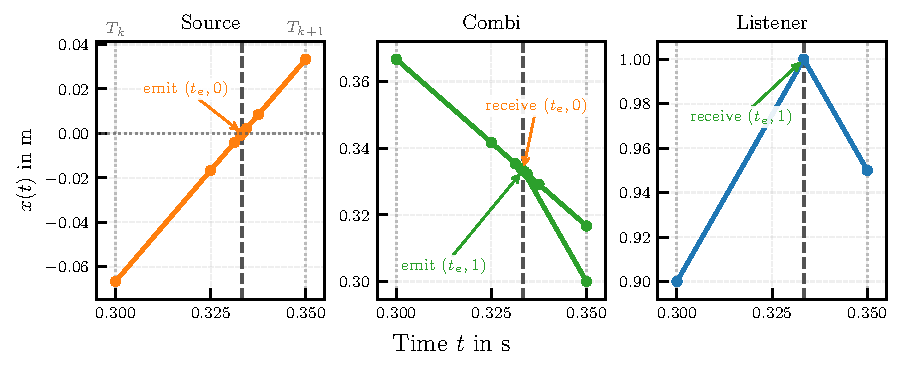
\includegraphics[width=\linewidth]{figures/5_implementation/hybrid/hybrid_event_chain.pdf}
    \caption{Event chain resolved with superdense time.
    The light dotted lines mark the original communication interval from $T_k = 0.30\,$s to $T_{k+1} = 0.35\,$s.
    The dark dashed line marks the localized event time inserted by the hybrid algorithm.
    The source emits the first event at $(t_e,0)$.
    The Combi component handles this event and emits a cascaded event at $(t_e,1)$.
    The Listener receives the cascaded event at the same physical time.}
    \label{fig:impl_hybrid_verification_chain}
\end{figure}

\paragraph{Strong event simultaneity and commutativity.}
The second scenario verifies the commutativity check that activates when two events reach the same listener at the same dense time.
Two \texttt{HybridSource} components are configured so that their zero-crossings coincide at the analytical time $t_e = \tfrac{2}{3}\,$s.
\texttt{Source\_1} has $x_1(t) = \tfrac{2}{3} - t$ with falling-edge direction.
\texttt{Source\_2} has $x_2(t) = -\tfrac{2}{3} + t$ with rising-edge direction.

A single \texttt{HybridListener} with initial velocity $v_0 = 3.0\,$m/s subscribes to both events and applies the updates $v \mapsto -v$ and $v \mapsto 2v$.
The two updates commute, so the final velocity must equal $-2\,v_0$ regardless of the dispatch order.

Figure~\ref{fig:impl_hybrid_verification_simultaneity} shows the located event time and the resulting listener trajectory.
The algorithm detects both crossings in the macro interval from $0.65$ to $0.70\,$s and locates them at the dense time $(t_e, 0)$ with $t_e \approx 0.66666667\,$s.
The post-event listener velocity is $-6.0\,$m/s, which matches the expected value $-2\,v_0$.

Listing~\ref{lst:hybrid_simultaneity_log} documents the commutativity dispatch.
Both events are grouped on the \texttt{Listener} and trigger a dynamic commutativity check because the listener does not declare commutativity through an annotation.
The check runs both handler permutations from a shared snapshot and confirms identical final states.
Both events are then dispatched at microstep $0$ through \texttt{System.dispatch\_event()}.

\begin{figure}[t]
    \centering
    \begin{subfigure}[t]{0.48\linewidth}
        \centering
        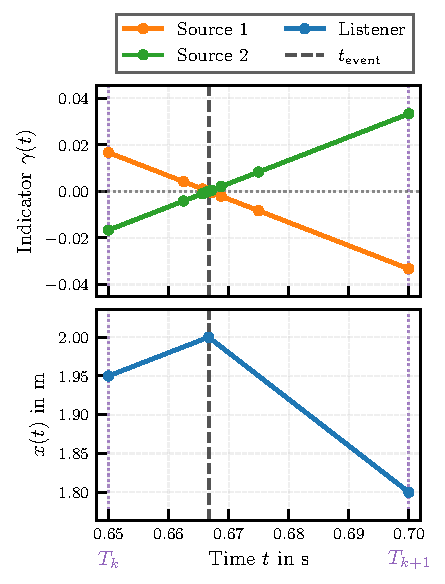
\includegraphics[width=\linewidth]{figures/5_implementation/hybrid/strong_simultaneity.pdf}
        \caption{Strong event simultaneity. Both sources cross zero at the same dense time $(t_e, 0)$ and the listener velocity is updated through commutative handlers.}
        \label{fig:impl_hybrid_verification_simultaneity}
    \end{subfigure}
    \hfill
    \begin{subfigure}[t]{0.48\linewidth}
        \centering
        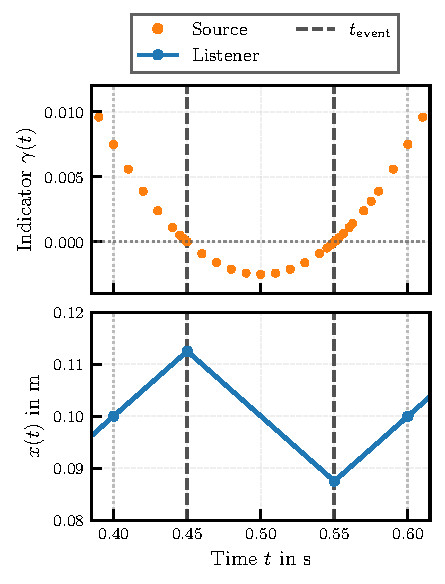
\includegraphics[width=\linewidth]{figures/5_implementation/hybrid/internal_event_reporting.pdf}
        \caption{Internal event reporting. The events at $t = 0.45\,$s and $t = 0.55\,$s lie strictly inside the macro interval $[0.4, 0.6]\,$s and are localized through internal hints.}
        \label{fig:impl_hybrid_verification_internal}
    \end{subfigure}
    \caption{Verification scenarios for two hybrid features that are not exercised in the case study. Dashed gray lines mark the localized event times; dotted gray lines mark the macro communication grid.}
    \label{fig:impl_hybrid_verification_pair}
\end{figure}


\begin{listing}[!htbp]
\begin{lstlisting}[
    basicstyle=\ttfamily\footnotesize,
    frame=single,
    backgroundcolor=\color{black!3},
    breaklines=true,
    columns=fullflexible,
    xleftmargin=0pt
]
Event crossing in [0.650000, 0.700000]: Source_1.v_invert, Source_2.v_double
Event located at t=0.66666667
Handling 2 event(s) at t=0.66666667, micro=0: Source_1.v_invert, Source_2.v_double
Events grouped by listener: {'Listener': ['v_invert', 'v_double']}
Checking commutativity for ['v_invert', 'v_double'] on Listener
Verifying commutativity dynamically for ['v_invert', 'v_double'] on Listener
Commutativity verified (dynamic): ['v_invert', 'v_double'] on Listener
\end{lstlisting}
\caption{Hybrid algorithm log for the strong-simultaneity scenario. Both crossings are localized at the same dense time, grouped on the listener, and confirmed commutative through the dynamic check before dispatch.}
\label{lst:hybrid_simultaneity_log}
\end{listing}

\paragraph{Internal event reporting.}
The third scenario verifies the internal-hint mechanism that allows components with internal micro-stepping to expose events between communication points.
An \texttt{EventReportingComponent} carries the indicator $h(t) = (t - T_1)(t - T_2)$ with roots $T_1 = 0.45\,$s and $T_2 = 0.55\,$s.
It steps internally with $\Delta t_{\mathrm{int}} = 0.01\,$s and reports an \texttt{InternalEventInfo} bracket whenever $h$ changes sign between two micro-steps.
An \texttt{EventListener} subscribes to the resulting \texttt{zero\_crossing} event and inverts its slope on every reception.
The macro step is set to $\Delta t = 0.2\,$s so that both roots fall strictly inside one macro interval.

The macro communication points alone cannot detect these events.
At both endpoints of the interval $[0.4, 0.6]\,$s the indicator is positive with $h(0.4) = h(0.6) = 0.0075$, so the trial-step detection of Section~\ref{sec:impl_hybrid_detection} would see no sign change.
The internal-hint mechanism resolves this by exposing the brackets $[0.44, 0.45]\,$s and $[0.54, 0.55]\,$s that the component records during its micro-steps.

Figure~\ref{fig:impl_hybrid_verification_internal} shows the indicator and the listener trajectory together with the macro grid.
The first hint narrows the bisection to $[0.44, 0.45]\,$s and the event is located at $t = 0.45\,$s.
The handler inverts the listener slope.
The second hint then narrows the bisection to $[0.54, 0.55]\,$s and the second event is located at $t = 0.55\,$s.
The two located event times agree with the analytical roots $T_1$ and $T_2$ within machine precision.

After the second event, a residual trial-step detection on $[0.55, 0.60]\,$s reports a rising crossing because the indicator at the new left boundary is below the sign tolerance.
The per-step deduplication cache rejects this detection since the time difference to the previously handled event is below \texttt{event\_dedup\_tol}.
%%%%%%%%%%%%%%%%%%%%%%%%%%%%%%%%%%%%%%%%%%%%%%%%%%%%%%%%%%%%%%%%
\section{Multi-Model Component}
\label{sec:impl_multi_model}

Runtime model switching allows one physical subsystem to use different internal models in different operating regimes.
The implementation realizes \ref{req:UR-09} and the derived requirements \ref{req:SR-09-01}--\ref{req:SR-09-04}.
The \texttt{MultiComponent} class implements this behavior as a component wrapper with a fixed external interface and one active internal model.
Section~\ref{sec:architecture_multicomponent} introduces the architectural roles of wrapper, mode selector, hysteresis, and state adapter.
The following subsections describe how \texttt{MultiComponent} realizes these roles.

%%%%%%%%%%%%%%%%%%%%%%%%%%%%%%%%%%%%%%%%%%%%%%%%%%%%%%
\subsection{Scope and Component Contract}
\label{sec:impl_multi_model_scope}

The \texttt{MultiComponent} class extends \texttt{CoSimComponent} with a registry of interchangeable internal models.
Each registered model is itself a \texttt{CoSimComponent}.
The surrounding \texttt{System} interacts only with the wrapper component.
It does not depend on the currently active internal model.

At runtime, exactly one model is active.
The wrapper identifies it through \texttt{active\_mode} and accesses it through \texttt{active\_comp}.
The active model performs the time step, provides the wrapper outputs, and serves as the source for state access and hybrid hooks.
Input assignment is handled separately, because incoming inputs are forwarded to the active model and cached for a possible later switch.
A user-defined \texttt{mode\_selector} may request a different mode before a step is executed.
On an accepted switch, the wrapper transfers the physical state from the current model to the target model.

Subclasses provide the model-specific parts of this process.
They register the available models and define how state is adapted between model interfaces.
Table~\ref{tab:multi_component_contract} summarizes the main contract.

\begin{table}[t]
  \centering
  \caption[Multi-component extension points.]{Main extension points and state fields of \texttt{MultiComponent}.}
  \label{tab:multi_component_contract}
  \begin{tabular}{lp{9.5cm}}
    \toprule
    \textbf{Element}                  & \textbf{Role}                                                                                                   \\
    \midrule
    \texttt{models}                   & Implements the model registry by storing available model implementations by mode key                            \\
    \addlinespace
    \texttt{active\_mode}             & Stores the key of the currently active model selected by the mode-switching wrapper                             \\
    \addlinespace
    \texttt{active\_comp}             & References the active component instance to which lifecycle and stepping calls are delegated                    \\
    \addlinespace
    \texttt{mode\_selector}           & Implements the mode selector by deriving the requested mode from the current time and selector-specific context \\
    \addlinespace
    \texttt{hysteresis}               & Implements the hysteresis support by blocking rapid switching when a dwell time is configured                   \\
    \addlinespace
    \texttt{\_allow\_mode\_switching} & Guards mode selection during trial steps and algebraic output evaluation                                        \\
    \addlinespace
    \texttt{\_adapt\_state()}         & Implements the state adapter by mapping the exported state to the target model interface                        \\
    \addlinespace
    \texttt{\_latest\_inputs}         & Caches the most recent external inputs so they can be replayed on the target model during a switch              \\
    \addlinespace
    \texttt{sync\_events}             & Records performed switches for inspection and debugging                                                         \\
    \addlinespace
    \bottomrule
  \end{tabular}
\end{table}

%%%%%%%%%%%%%%%%%%%%%%%%%%%%%%%%%%%%%%%%%%%%%%%%%%%%%%
\subsection{Initialization and Interface Unification}
\label{sec:impl_multi_model_initialization}

A concrete subclass registers its internal models during construction.
It stores them in \texttt{models}, selects the initial model through \texttt{active\_mode}, and stores the corresponding component in \texttt{active\_comp}.
The subclass then calls \texttt{\_unify\_ports()} before the wrapper is registered with a \texttt{System}.
This construction-time setup is required because signal connections are validated before component initialization.

The wrapper must expose one stable port interface to the surrounding system.
For this purpose, \texttt{\_unify\_ports()} adopts the input and output specifications of the active component.
It then checks that every registered model provides compatible ports with the same names, directions, port types, and units.
If a model misses a required port or exposes an incompatible specification, construction fails with a \texttt{ValueError}.
This ensures that a later mode switch cannot change the external interface of the component.

Direct-feedthrough metadata must also remain fixed.
The wrapper compares the feedthrough dictionaries of all registered models during initialization.
A mismatch is rejected.
Section~\ref{sec:impl_structural} assumes fixed zero-delay behavior for every component during a simulation run.
The \texttt{MultiComponent} class can therefore switch models only when the externally visible dependency structure remains unchanged.

%%%%%%%%%%%%%%%%%%%%%%%%%%%%%%%%%%%%%%%%%%%%%%%%%%%%%%
\subsection{Runtime Model Switching}
\label{sec:impl_multi_model_switching}

Runtime switching is part of the component step.
When a master algorithm calls \texttt{do\_step(t, dt)} on the wrapper, the base component logic delegates to \texttt{\_do\_step\_internal(t, dt)}.
Zero-duration calls are treated as output-refresh evaluations.
They are delegated to the current active model without mode selection.
For positive step sizes, the wrapper first checks the switching guards.
Mode selection is skipped when switching is disabled, when no selector is configured, or when the hysteresis dwell window is active.
The selector is evaluated only after these guards pass.
Figure~\ref{fig:impl_multi_model_switching} summarizes the switching path.

\begin{figure}[t]
  \centering
  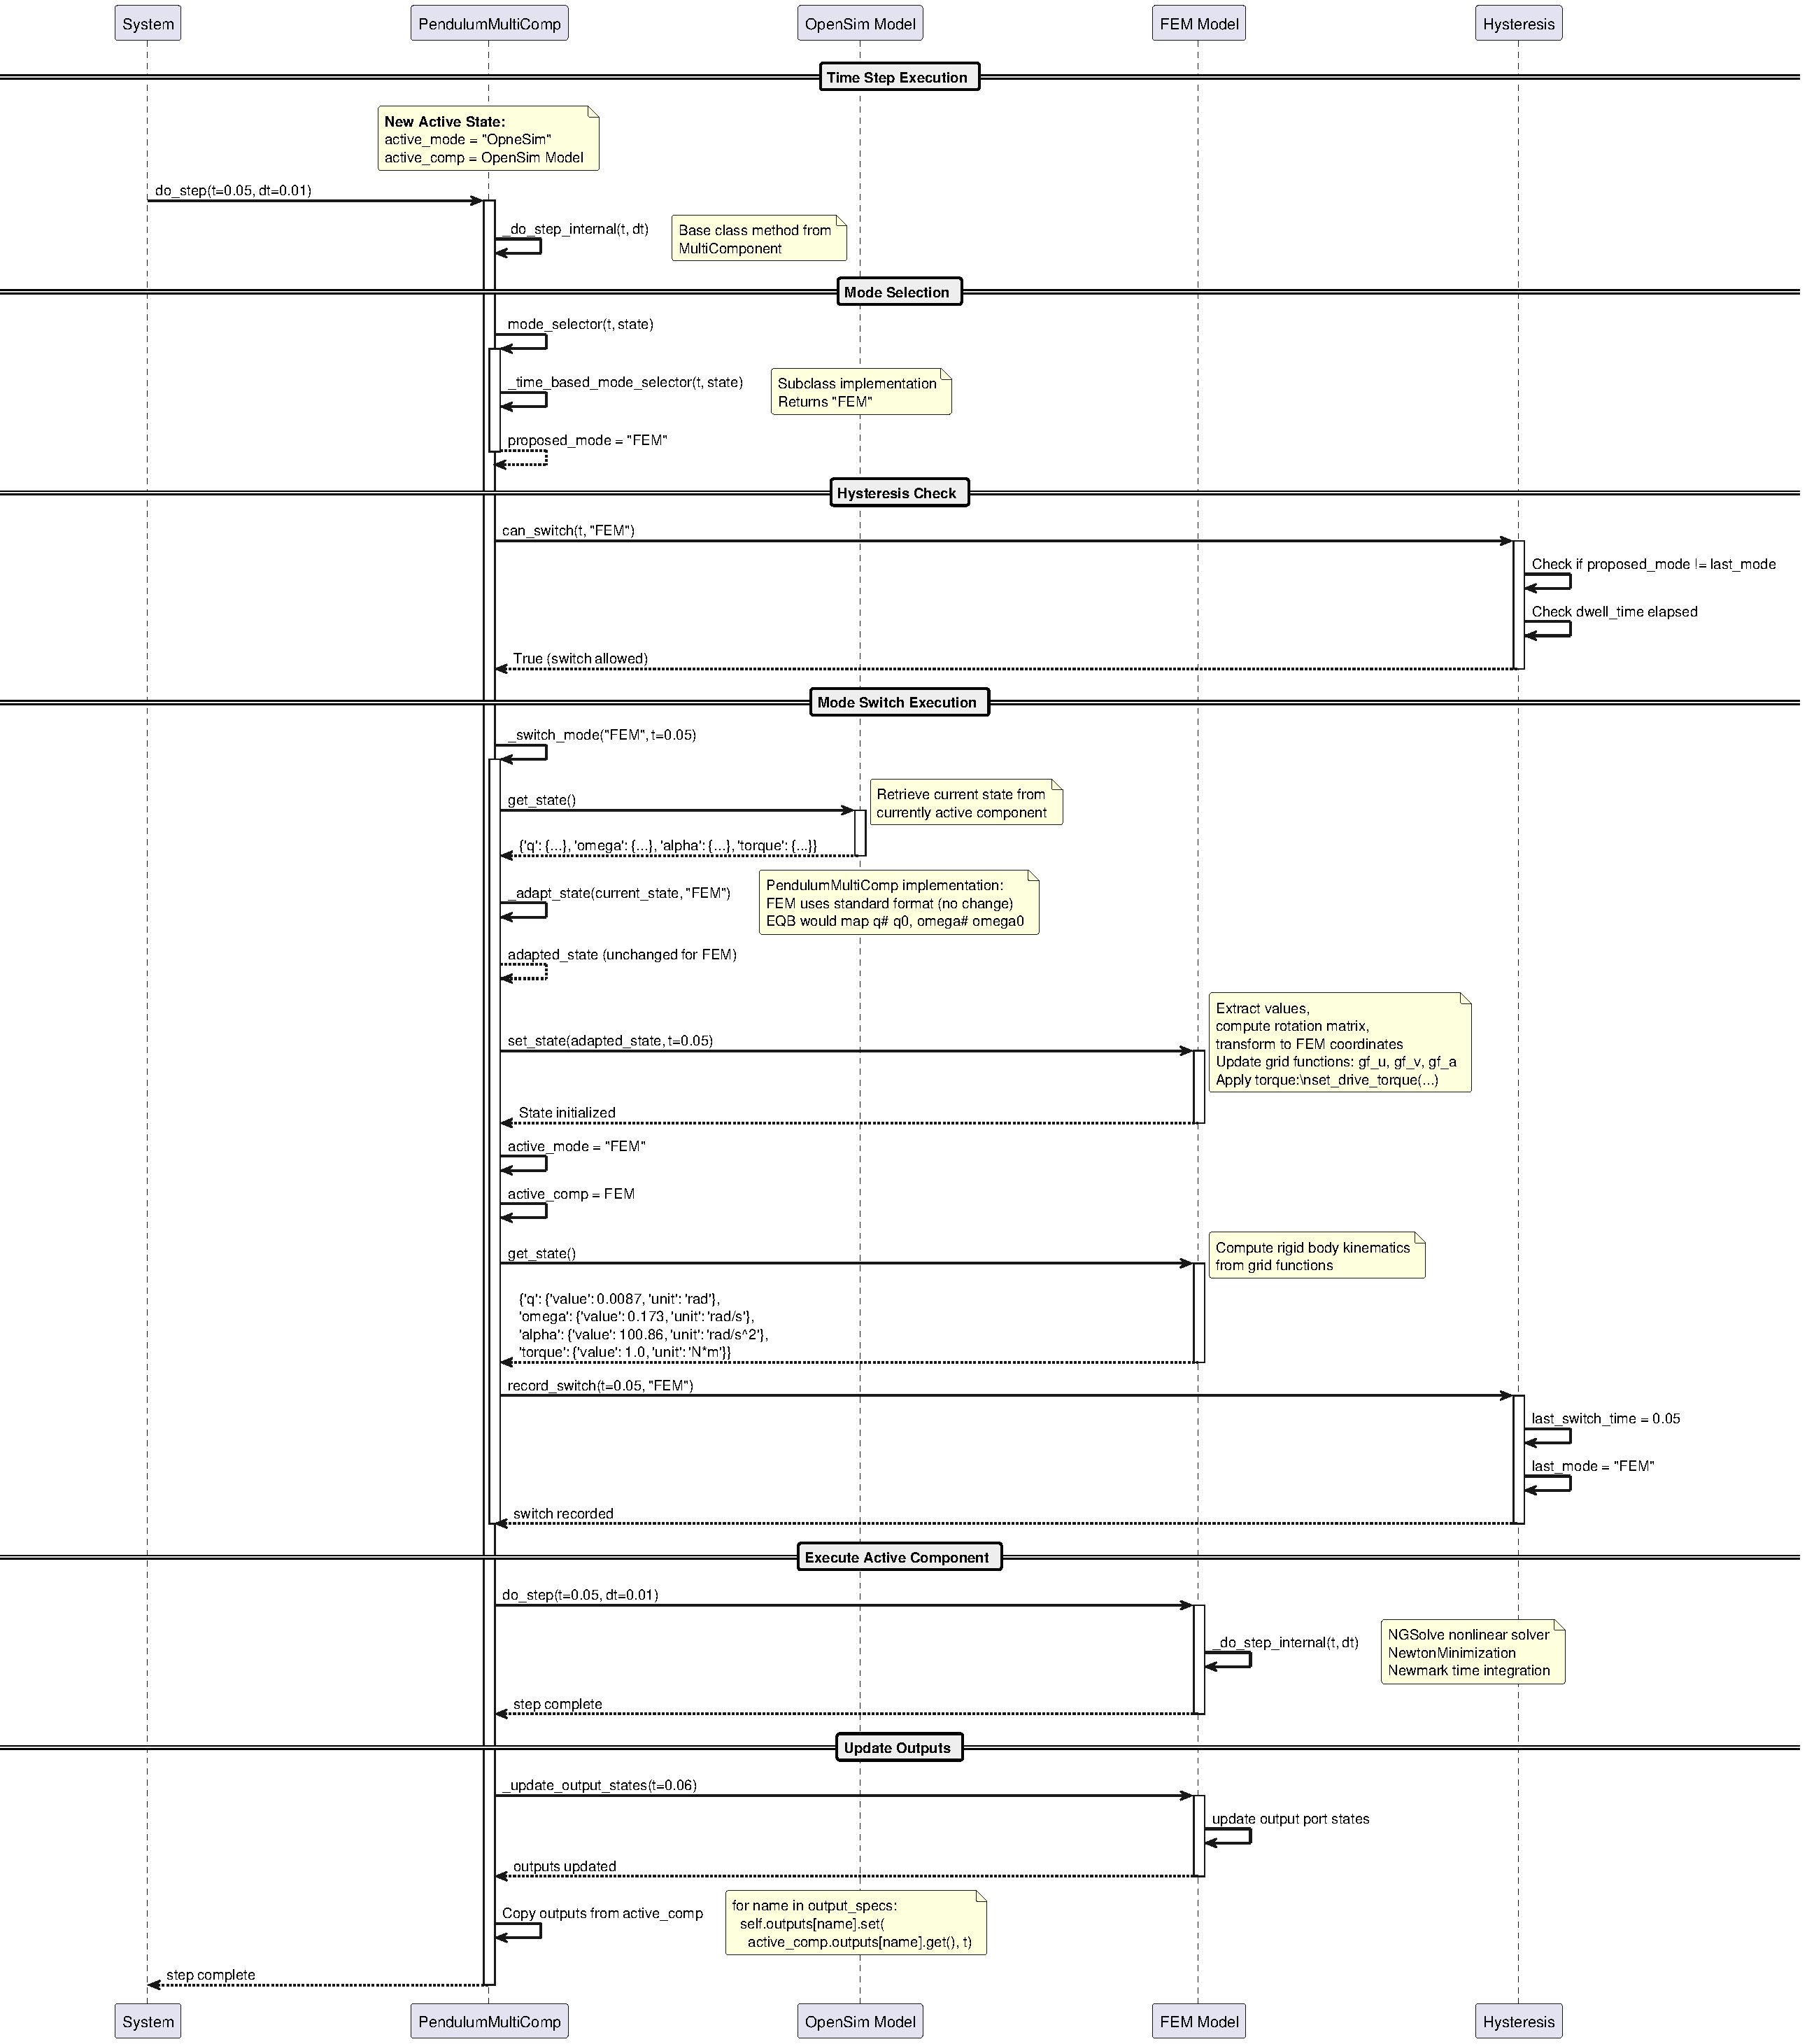
\includegraphics[width=\textwidth]{diagrams/out/pdf/execution/MultiComponent_Switching.pdf}
  \caption[Runtime switching sequence.]{Runtime switching sequence of the \texttt{MultiComponent} class for a positive macro step.
  The wrapper applies switching guards, transfers state and cached inputs on an accepted switch, and delegates the step to the active model.}
  \label{fig:impl_multi_model_switching}
\end{figure}

A configured \texttt{Hysteresis} object may block a requested switch.
During the dwell window, the wrapper keeps the current mode and does not call the selector.
Outside the dwell window, the selector returns the requested mode.
If the requested mode equals the current mode, the wrapper keeps the current model for this step.
This prevents rapid switching near decision boundaries.

If the requested mode is accepted, \texttt{\_switch\_mode()} performs the transition.
It first retrieves the current state from the active model.
The state is then passed to \texttt{\_adapt\_state()}.
This hook maps the state to the format expected by the target model.
The adapted state is written to the target component through \texttt{set\_state()}.
The wrapper then updates \texttt{active\_mode} and \texttt{active\_comp}.

Each accepted switch is stored in \texttt{sync\_events}.
The stored entry contains the switch time and the two involved modes.
Detailed source and target state snapshots are recorded only when \texttt{record\_switch\_state} is enabled.
This log is used to inspect whether the state transfer behaved as expected.

After the optional mode switch, the actual time step is delegated to the active component through \texttt{do\_step(t, dt)}.
The master algorithm therefore does not need a special execution path for multi-model components.
The internal mode selection remains encapsulated inside the wrapper.
Section~\ref{sec:impl_multi_model_state_events} describes how input forwarding, output propagation, and hybrid delegation are handled around the active model.

%%%%%%%%%%%%%%%%%%%%%%%%%%%%%%%%%%%%%%%%%%%%%%%%%%%%%%
\subsection{Input, Output, and Hybrid Delegation}
\label{sec:impl_multi_model_state_events}

The \texttt{set\_inputs()} method forwards incoming values to the active model and stores them in \texttt{\_latest\_inputs}.
Inactive models are not advanced and do not receive every input update.
During an accepted switch, the cached inputs are replayed on the target model before the adapted state is written.
The target model is therefore synchronized with the most recent external inputs at the switch time.

Output propagation follows the opposite direction.
After the active model has advanced, \texttt{\_update\_output\_states()} copies the active model outputs to the wrapper ports.
The surrounding \texttt{System} therefore reads outputs only from the \texttt{MultiComponent}.
Event ports are handled in the same update step.
Ports corresponding to triggered events are set to \texttt{True}, while inactive event ports are reset to \texttt{False}.

Algebraic output evaluation uses the same active-model delegation.
The wrapper temporarily disables runtime model switching during \pyfn{evaluate\_outputs()}.
It evaluates the active model for the supplied trial inputs.
The resulting values are copied to the wrapper ports.
This prevents direct-feedthrough detection from changing the active model.
It also prevents \ac{IJCSA} residual evaluations from changing the active model.

State access is routed through the active model.
The \texttt{get\_state()} method returns the state of \texttt{active\_comp}.
The \texttt{set\_state()} method adapts the provided state to the active mode and writes it to \texttt{active\_comp}.
The wrapper therefore provides one access point.
The concrete state schema remains defined by the active model and the subclass adaptation logic.

The hybrid hooks are delegated to the active model as well.
Event indicator evaluation, crossing detection, rollback snapshots, event handling, and internal event hints are forwarded to \texttt{active\_comp}.
Runtime model switching can be disabled through \texttt{\_allow\_mode\_switching}.
The hybrid algorithm uses this flag during trial steps.
Event detection and localization therefore cannot change the active model while a rollback snapshot is valid.

%%%%%%%%%%%%%%%%%%%%%%%%%%%%%%%%%%%%%%%%%%%%%%%%%%%%%%
\subsection{Verification}
\label{sec:impl_multi_model_verification}

The verification scenario isolates the switching mechanism through a two-mode integrator with a known analytical reference.
The wrapper holds two scalar integrators that share the input and output interface but apply different gains to the constant input $u = 1$.
Mode~A integrates with $k_A = 1.0$ and Mode~B with $k_B = 2.0$.
Both models share the state variable $x$ with $x(0) = 0$.
A \texttt{mode\_selector} switches from Mode~A to Mode~B at the analytical time $t_s = 0.5\,$s.

The expected trajectory is piecewise linear with slope $k_A$ before the switch and slope $k_B$ after.
The state must remain continuous at $t_s$, since \texttt{\_switch\_mode()} adapts and transfers the active state to the target model before the next time step.

Figure~\ref{fig:impl_multi_model_verification} compares the numerical trajectory with the analytical reference and shows the active mode over time.

\begin{figure}[!htbp]
  \centering
  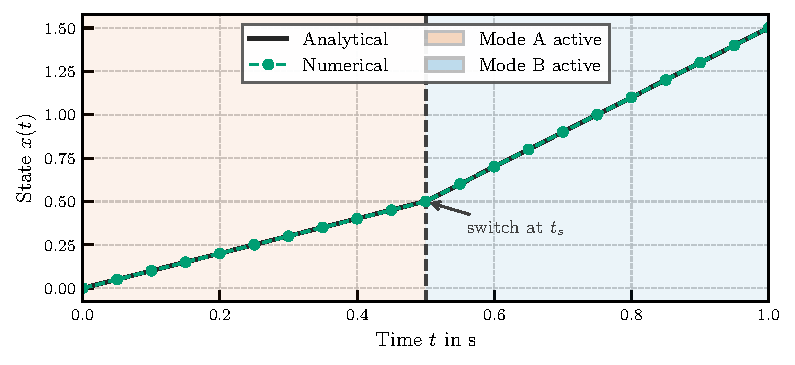
\includegraphics[width=0.82\linewidth]{figures/5_implementation/multi_component/multi_component_switching_verification.pdf}
  \caption[Two-model integrator check for runtime model switching]{Two-model integrator check for runtime model switching.
    The trajectory follows the analytical reference and remains continuous at the accepted switch time.}
  \label{fig:impl_multi_model_verification}
\end{figure}

The numerical trajectory matches the analytical solution within machine precision.
The maximum absolute error is $3.3\cdot 10^{-16}$.
The active mode changes from A to B exactly at $t_s$.
The recorded \texttt{sync\_events} entry confirms one accepted switch with retrieved and synchronized states equal to $x(t_s)=0.5$.
The hysteresis path is covered by the unit tests and is not repeated here.

The preceding sections verify the main framework features in isolation.
Together, these features provide the executable basis for heterogeneous co-simulation scenarios with structural analysis, algebraic-loop resolution, hybrid event handling, and runtime model switching.
The next chapter evaluates their combined use in the controlled-pendulum case study.
The focus therefore shifts from feature-level verification to system-level validation against the reference simulation and the intended application workflow.